%% Version 4.3.2, 25 August 2014
%
%%%%%%%%%%%%%%%%%%%%%%%%%%%%%%%%%%%%%%%%%%%%%%%%%%%%%%%%%%%%%%%%%%%%%%
% Template.tex --  LaTeX-based template for submissions to the 
% American Meteorological Society
%
% Template developed by Amy Hendrickson, 2013, TeXnology Inc., 
% amyh@texnology.com, http://www.texnology.com
% following earlier work by Brian Papa, American Meteorological Society
%
% Email questions to latex@ametsoc.org.
%
%%%%%%%%%%%%%%%%%%%%%%%%%%%%%%%%%%%%%%%%%%%%%%%%%%%%%%%%%%%%%%%%%%%%%
% PREAMBLE
%%%%%%%%%%%%%%%%%%%%%%%%%%%%%%%%%%%%%%%%%%%%%%%%%%%%%%%%%%%%%%%%%%%%%

%% Start with one of the following:
% DOUBLE-SPACED VERSION FOR SUBMISSION TO THE AMS
\documentclass{ametsoc}

% TWO-COLUMN JOURNAL PAGE LAYOUT---FOR AUTHOR USE ONLY
% \documentclass[twocol]{ametsoc}

%%%%%%%%%%%%%%%%%%%%%%%%%%%%%%%%
%%% To be entered only if twocol option is used

\journal{mwr}

%  Please choose a journal abbreviation to use above from the following list:
% 
%   jamc     (Journal of Applied Meteorology and Climatology)
%   jtech     (Journal of Atmospheric and Oceanic Technology)
%   jhm      (Journal of Hydrometeorology)
%   jpo     (Journal of Physical Oceanography)
%   jas      (Journal of Atmospheric Sciences)	
%   jcli      (Journal of Climate)
%   mwr      (Monthly Weather Review)
%   wcas      (Weather, Climate, and Society)
%   waf       (Weather and Forecasting)
%   bams (Bulletin of the American Meteorological Society)
%   ei    (Earth Interactions)

%%%%%%%%%%%%%%%%%%%%%%%%%%%%%%%%
%Citations should be of the form ``author year''  not ``author, year''
\bibpunct{(}{)}{;}{a}{}{,}

%%%%%%%%%%%%%%%%%%%%%%%%%%%%%%%%

%%% To be entered by author:

%% May use \\ to break lines in title:

\title{Assessing Adaptive Mesh Refinement (AMR) in a Forced Shallow Water Model with Moisture}

%%% Enter authors' names, as you see in this example:
%%% Use \correspondingauthor{} and \thanks{Current Affiliation:...}
%%% immediately following the appropriate author.
%%%
%%% Note that the \correspondingauthor{} command is NECESSARY.
%%% The \thanks{} commands are OPTIONAL.

    %\authors{Author One\correspondingauthor{Author One, 
    % American Meteorological Society, 
    % 45 Beacon St., Boston, MA 02108.}
% and Author Two\thanks{Current affiliation: American Meteorological Society, 
    % 45 Beacon St., Boston, MA 02108.}}

\authors{Jared O. Ferguson\correspondingauthor{Department of Climate and
Space Sciences and Engineering, University of Michigan, 2455 Hayward,
Ann Arbor, MI 48109, USA} and Christiane Jablonowski}

%% Follow this form:
    % \affiliation{American Meteorological Society, 
    % Boston, Massachusetts.}

\affiliation{Department of Climate and Space Sciences and Engineering,
University of Michigan, Ann Arbor, Michigan}

%% Follow this form:
    %\email{latex@ametsoc.org}

\email{joferg@umich.edu}

%% If appropriate, add additional authors, different affiliations:
    %\extraauthor{Extra Author}
    %\extraaffil{Affiliation, City, State/Province, Country}

\extraauthor{Hans Johansen, Peter McCorquodale}
\extraaffil{Lawrence Berkeley National Laboratory, Berkeley,
California}



%%%%%%%%%%%%%%%%%%%%%%%%%%%%%%%%%%%%%%%%%%%%%%%%%%%%%%%%%%%%%%%%%%%%%
% ABSTRACT
%
% Enter your abstract here
% Abstracts should not exceed 250 words in length!
%
% For BAMS authors only: If your article requires a Capsule Summary, please place the capsule text at the end of your abstract
% and identify it as the capsule. Example: This is the end of the abstract. (Capsule Summary) This is the capsule summary. 

\abstract{Two nonlinear forced shallow water test cases are implemented in a fourth-order finite volume dynamical core with adaptive mesh refinement (AMR) to investigate AMR�s ability to track and resolve complex evolving features. Traditional shallow water test cases consists mainly of large-scale smooth flows that do not effectively test the multiscale abilities of variable resolution and AMR models to resolve sharp gradients and small-scale flows. Adding forcing mechanisms to the shallow water system to model key atmospheric processes adds complexity and creates small-scale dynamic features of interest that can serve as foci for dynamic refinement, while remaining simple enough to study key numerical components of a model�s dynamical core. The two shallow water forced test cases implemented in this paper are a strengthening vortex formed by convection-like forcing and a barotropic jet implemented in a moist-thermodynamic phase change model that triggers front-like cloud and precipitation features. Both test cases were run with a series of uniform resolutions and a variety of AMR tagging criteria. Key features in both test cases have a high sensitivity to model resolution but also structurally converge at high resolutions. The AMR simulations demonstrated that refinement can resolve key local features without requiring global high-resolution grids but results were sensitive to the refinement criteria. Criteria that triggered refinement early in a simulation performed the best while criteria that delayed refinement for several days required careful tuning of thresholds to improve results compared with uniform resolution simulations.
}

\begin{document}

%% Necessary!
\maketitle


%%%%%%%%%%%%%%%%%%%%%%%%%%%%%%%%%%%%%%%%%%%%%%%%%%%%%%%%%%%%%%%%%%%%%
% MAIN BODY OF PAPER
%%%%%%%%%%%%%%%%%%%%%%%%%%%%%%%%%%%%%%%%%%%%%%%%%%%%%%%%%%%%%%%%%%%%%
%

%% In all cases, if there is only one entry of this type within
%% the higher level heading, use the star form: 
%%
% \section{Section title}
% \subsection*{subsection}
% text...
% \section{Section title}

%vs

\section{Introduction}
The spherical shallow water equations serve as an effective test bed for 
assessing numerical methods for general circulation models (GCMs). They 
exhibit many of the dynamics and complexities of the full 3D equations with 
the advantage of being two-dimensional and thus less computationally intensive.  
Full 3D models use the dycore of the GCM with
 a plethora of sub-grid parameterization 
schemes for unresolved physical and thermodynamical processes, further 
adding to their complexity.  However, shallow water-type models and 
the unforced test cases traditionally associated with them \citep{Williamson:1992kx}
are missing features (e.g. water vapor, convection, latent heat release, 
thermal forcing) which play key roles in atmospheric and 
climatological phenomena. Including simplified forcing mechanisms to represent 
such moisture and heating
processes in the shallow 
water system narrows the gap between idealized unforced studies 
and full-physics models. These forced shallow water 
models include the dynamical complexities of the full models and can retain
the non-linearity of the physical processes.  However,
the shallow water equations are still simple enough to effectively study
the key components of the dycore such as the numerical algorithms,
computational grid, and, for variable resolution and AMR models, grid refinement
strategies and efficacy. Shallow water models have the added advantage of being
computationally cheap to run at high resolutions.

A variety of studies have implemented forcing in shallow water models to study
 the fundamental dynamical aspects of large synoptic
scale climatological features, such as the Madden-Julian Oscillation (MJO),
as well as intense, small-scale features including tropical cyclone 
evolution, cumulus convection, and frontal propagation.
\cite{ferreira1996dynamical} and \cite{yang2013triggered} implement
spatially and temporally varying mass sinks and sources within nonlinear 
shallow-water models to simulate MJO convection in studies of MJO
induced twin tropical cyclones and MJO convective envelope 
development, respectively. In \cite{enagonio2001tropical}, 
the authors examined tropical cyclogenesis
by forcing a shallow water system with periodic pulses of vorticity to represent multi-burst convection.
 \cite{hendricks2014hurricane} mimicked diabatic heating in hurricane 
eyewalls within a Cartesian shallow water model by using a prescribed annular
 axisymmetric mass sink.

A framework to study the specific dynamical role of moist processes in a shallow water system
was proposed in the seminal work by \cite{gill1982studies}. In this system,
 a moisture equation with nonlinear precipitation thresholds was added to the 
linearized shallow-water equations to model the effects of latent heat release on the 
propagation of large scale disturbances. Similar models incorporating this framework for 
parameterizing moisture were analyzed by \cite{goswami1991modification} in the context of
large-scale equatorial wave propagation and by \cite{frierson2004large},
\cite{stechmann2006structure}, and \cite{bouchut2009fronts} in studies of tropical precipitation 
fronts. Unlike the other studies mentioned, \cite{bouchut2009fronts} implements the moist-convective 
parameterizations in a fully nonlinear rotating shallow water model,
also used by \cite{lambaerts2011moist} to compare the differences in barotropic instability evolution between moist and dry conditions. To study the
dynamical role of moisture in tropical cyclone instabilities, \cite{lahaye2016understanding} 
also used this moist rotating shallow-water model with an added evaporation 
mechanism. \cite{rostami2017influence} implemented both a 1-level barotropic 
version and a 2-level shallow water baroclinic version of the model introduced in 
\cite{lambaerts2011moist} to study large-scale small Rossby number vortices.

Other frameworks for simulating precipitation and convection in the shallow water
system that have been implemented recently included models by 
\cite{wursch2014simple} and \cite{zerroukat2015moist}.
\cite{wursch2014simple} developed a simplified model of cumulus convection 
incorporating representation of updrafts, downdrafts, and idealized precipitation 
effects in a 1D shallow water model. 
Once the fluid exceeds a certain threshold height, signaling the 
onset of convection, mechanisms serving as simplified representations 
of cumulus convection modify the geopotential height to create
conditional instability and mimic updrafts. 
This method was extended to a rotating, 2D shallow 
water model in \cite{kent2017dynamics}.
In \cite{zerroukat2015moist}, the authors re-derived the two-dimensional
shallow water system from the three-dimensional moist Boussinesq 
approximation. Density was permitted to vary with temperature,
resulting in additional buoyancy related terms in the momentum equations and
permitting a dynamics-moisture feedback. \cite{zerroukat2015moist} also 
implemented a three-state moisture model consisting of vapor, cloud, and 
precipitated species.

In this paper, we implement two forcing frameworks that seek to mimic moisture 
and convection in a spherical, 2D shallow water system. In the first, 
 moist shallow water equations derived in \cite{bouchut2009fronts} and 
\cite{lahaye2016understanding} cause
 convective forcing and precipitation, which induce TC-like vortices to develop and strengthen. In the second 
framework, the barotropic instability shallow water test case of 
\cite{galewsky2004initial} is implemented within a different moist shallow water system developed from 
 \cite{zerroukat2015moist}. As the jet becomes unstable and collapses, front-like 
 systems containing clouds and precipitation develop. Using these frameworks, we
 investigate the distinctive dynamics produced by the non-linear physics processes
 within the traditional shallow water system. A main goal of this paper is to
 introduce test cases with more challenging complex and transient features
 to test the ability of adaptive mesh refinement (AMR) 
 to track and resolve these moving and growing features.
 
 We use the fourth-order finite-volume Chombo AMR model
 presented in \cite{mccorquodale2015adaptive} and
 \cite{ferguson2016analyzing} for the 2D shallow water equations. 
 This model implements dynamic refinement using
 a mapped-multiblock AMR technique which overlays the base grid with more refined patches.
 Using AMR, we observe how features in the test cases evolve due to the forcing 
 processes and how those forcing processes are affected by the AMR refinement. 
Ideally, the physics forcing schemes should be able to effectively span 
the multiple levels of refinement and changing resolutions created by AMR.
 In addition, we seek to quantify improvements gained from AMR grids
 and determine effective refinement criteria.

This paper is organized as follows. Section \ref{sec:modelintro} provides a brief overview
of the finite volume model and the Chombo multiblock AMR techniques.
Section \ref{sec:forcedvort} describes the shallow water equations
with moist convective forcing and the strengthening vortex test case.
Section \ref{sec:wetvortresults} compares numerical results of the strengthening vortex
test case for uniform and AMR runs of varying resolution. The
 \cite{zerroukat2015moist} moist shallow water system with
 barotropic instability test case and its numerical results
 are presented in Section \ref{sec:kesslersw}.  Section \ref{sec:conclusion2} summarizes our
 conclusions from the two test cases.

\section{High-Order Finite-Volume Chombo AMR Model}
\label{sec:modelintro} 
  For this study we employ an unstaggered finite-volume (FV) mapped-multiblock 
  dynamical core (dycore) that is fourth-order accurate and adaptive in both 
  space and time. The model's AMR is based on the Chombo AMR 
  library \citep{Adams:2015gd} and an in-depth description of the model 
  dynamical core for the shallow-water equations on an equiangular cubed-sphere 
  grid can be found in \cite{mccorquodale2015adaptive}. 
  The model uses a classical fourth-order Runge-Kutta (RK4) 
  time discretization scheme. In the spatial domain, fourth-order 
  accurate finite-volume discretization is implemented to compute 
  flux averages on the faces of each cell. 
  Additionally, a sixth-order 
  diffusive operator is applied to smooth the flux calculations while still 
  maintaining the scheme's fourth-order accuracy. The model is mass 
  conserving and conserves energy up to the temporal truncation error, when 
  limiters or explicit dissipation are not applied. 
  
  The cubed-sphere grid consists of a cube whose six separate panels are 
  projected onto the surface of a sphere. In addition to eliminating the polar 
  singularities found in spherical latitude-longitude grids, the equiangular cubed-sphere 
  also leads to a quasi-uniform mesh with similarly sized grid cells across the sphere. 
  The discrete resolution of the cubed-sphere grid is denoted by $c\{N_c\}$ 
  where $N_c$ is the number of grid cells in each direction on a panel. Several 
  properties of the equiangular cubed-sphere grid, including approximate grid 
  spacings, are given in Table~\ref{tb:grids2} for resolutions used in this paper.
   
  Our mapped-multiblock AMR approach implements a hierarchy of 
  nested grid levels of increasing resolution. 
  \cite{mccorquodale2015adaptive} and \cite{ferguson2016analyzing} 
  both provide a detailed descriptions of the AMR technique. 
  The grid resolution of an AMR level is defined by its refinement ratio 
  to the grid resolution of the coarser level below it. Finer levels are 
  placed over regions where coarse cells have been marked (tagged) 
  by the model as meeting the refinement criterion. The cell values in 
  the finer level are initialized via interpolations from the coarser level. 
  Ghost cells are used to calculate fluxes at the level boundaries in the 
  same manner as is done at the cubed-sphere panel boundaries. If 
  multiple levels are used, intermediate levels must cover enough area 
  to ensure that the finer level is nested within the intermediate level; it 
  is required that the ghost cells for the finer level are only interpolated 
  from cells within the intermediate level.  
  
  Finer levels are sub-cycled in time to maintain a constant Courant 
  number across all resolutions. The sub-cycling routine can be 
  summarized as follows: after interpolating values to the refined 
  level, the coarser level is advanced by one time step. The finer level 
  is then advanced in time using a smaller time step determined by 
  dividing the coarse time step by the refinement ratio between the two 
  levels.  At each finer time step, the ghost cells used to calculate the 
  boundary fluxes at the finer level's edges are updated via a temporal 
  interpolation from the RK4 method. After the sub-cycling is complete, 
  the values on the coarse grid are updated from the solution on the 
  finer grid.  
  
  The refinement criteria determine the regions over which additional 
  grid levels are placed based on user-selected threshold values for 
  flow properties.  The thresholds are set independently for each 
  simulation and their criteria can be based on a variety of properties, 
  such as tracer values, gradients, relative vorticity, or a combination of 
  these. The AMR dycore can incorporate multiple levels of refinement, 
  preset for each simulation, and tagging criteria can be uniformly 
  enforced across all levels or required to scale with increasing resolution.
 
%--------Section 
\section{Convectively forced shallow water vortices}
\label{sec:forcedvort} 
  This test cases simulates the growth and development of TC-like 
  vortices in a 2D shallow water framework using a moist convective forcing 
  mechanism. Weak vortices are initialized on a calm background field 
  of uniform height. Evaporation and precipitation cause these vortices to strengthen. 
  After several days of strengthening, the orderly vortices collapse and a more chaotic 
  system evolves, characterized by several smaller vortices and jet-like background flow. 

  We first provide a description of the moist convective shallow water system 
  and an overview of the initial conditions. Next we present the evolution of an 
  isolated vortex in this test case at a uniform high resolution. Then we demonstrate
  the use of AMR in this test case comparing the affects of different resolutions and
  various tagging criteria.

%Subsection
  \subsection{``Moist-convective`` shallow water equations }
     The shallow water equations are modified to include the transport of a 
     moisture variable and the effects of moist convection, precipitation, and evaporation. 
     We extend the forcing schemes developed by \cite{bouchut2009fronts} and 
     \cite{lahaye2016understanding} to the 2D shallow water equations on the sphere. 
     \cite{bouchut2009fronts} developed a moist convective scheme 
     for a rotating shallow water model to study precipitation fronts. 
     It only included an advected moisture variable, precipitation, and 
     a convection mimicking process, while \cite{lahaye2016understanding} 
     added an evaporation forcing to the system.  
     
     In this moist convective system, a relaxation sink is added to the moisture equation (Eq. \ref{eq:swqcon}), 
     representing precipitation when moisture levels exceed a saturation value. 
     A corresponding convective mass sink is added to the continuity equations and a 
     moisture source is added to the moisture equation to represent evaporation. 
     The equations for this modified shallow water system are
   \begin{equation}
     \label{eq:swmomf} \frac{\partial h \mathbf{v}}{\partial t} +
     \nabla \cdot ( h \mathbf{v} \mathbf{v}) + f \mathbf{\hat{k}}\times(h\mathbf{v}) + gh\nabla H = 0
   \end{equation}
   \begin{equation}
     \label{eq:swconf}  \frac{\partial h}{\partial t} + \nabla \cdot (h\mathbf{v}) = - \beta P 
   \end{equation}
   \begin{equation}
     \label{eq:swqcon}  \frac{\partial hQ}{\partial t} + \nabla \cdot (hQ\mathbf{v}) = h(E - P).
   \end{equation}
   Here $\mathbf{v}$ is the velocity vector, $\mathbf{v}\mathbf{v}$ denotes the outer product
   of the velocity vector, $f$ is the Coriolis parameter, $g$ is 
   the acceleration due to gravity,
   $h$ is the height of the fluid, $H$ is the total height including topography, and the
   dimensionless moisture variable $Q$ represents bulk humidity. 
   $E$ is the evaporation in the moisture budget and $P$ is the precipitation. 
   The latent heat release from precipitation does not directly influence the 
   horizontal momentum. It is instead linked to convective vertical velocity 
   directly proportional to $P$ at the upper surface of the fluid.
   Since this system is designed to represent only the lower part of the 
   troposphere, the convective updraft can be constructed as a mass exchange 
   from this surface layer. The mass exchange is then represented as a mass 
   sink in Equation \ref{eq:swconf} governed by an adjustable
   constant $\beta$.  A detailed explanation for the implementation is 
   presented by \cite{bouchut2009fronts}.

   The precipitation sink is calculated in terms of $Q$ and the saturation value $Q_s$,
   \begin{equation}
     \label{eq:precip} P = \frac{Q-Q_s}{\tau}\mathbf{H}(Q-Q_s).
   \end{equation}
   with a relaxation time of $\tau$. $\mathbf{H}(\cdot)$ is the Heaviside function
    so that $P = 0$ whenever $Q \leq Q_s$.
   A common parameterization used in \cite{lahaye2016understanding} is modified
   to include an upper velocity limit on the evaporation rate, thus the evaporation rate $E_r$ becomes
   %\begin{equation}
     \begin{align}
        \label{eq:evap} 
     &E_r  =   \alpha_e  \lvert \vec{v} \rvert & \mathrm{for} \ \lvert \vec{v} \rvert < v_\mathrm{max} \nonumber \\
     &E_r  =   \alpha_e (v_\mathrm{max}) &  \mathrm{for} \ \lvert \vec{v} \rvert > v_\mathrm{max} 
     \end{align}
   %\end{equation} 
   where the evaporated moisture is dependent on the magnitude of the 
   velocity $\vec{v}$ and the adjustable coefficient $a_e$. This evaporation scales 
   with wind speed until $v_{\mathrm{max}}$. In the simulations presented below,
   $a_e = 0.055$ m$^{-1}$ and $v_{\mathrm{max}} = 30$ m s$^{-1}$.
   At higher velocity magnitudes, $E_r$ is constant.
   
   As established, evaporation is unlimited, but such a setup can lead to runaway 
   supersaturation and very large height forcing which causes exceedingly high wind 
   velocities and negative height values in longer simulations.
   To limit these sources of instability, we refine the forcing mechanics with the following additional mechanisms.
   We add a moisture reservoir from which the evaporation is drawn. This reservoir is a simplistic representation of
   ocean surface heat content and its limiting effects on tropical convection and tropical cyclone intensity.
   In this forcing scheme, the evaporation rate $E_r$ defined in Eq. \ref{eq:evap} draws moisture from the finite reservoir 
    $C_r(\phi,\lambda)$. However, evaporation cannot exceed the amount
    of moisture remaining in $C_R$ for any given latitude-longitude $(\phi,\lambda)$ point in space and time.
    Thus, the evaporation rate $E$ applied in Eq. \ref{eq:swqcon} is capped so that
    \begin{equation}
      \label{eq:crlimit}
         E = \frac{1}{\Delta t}\min\left(E_r \Delta t, C_r\right)
    \end{equation}
   where $\Delta t$ is the model time step. So the evaporation 
   rate becomes zero if there is no longer moisture to be drawn from $C_r$.

    The amount of moisture in the reservoir is affected by
    evaporation which removes moisture from 
    the reservoir, and a Newtonian relaxation slowly returns the reservoir to its initial state. 
    The rate of change of moisture in the reservoir is
    \begin{equation}
        \label{eq:ocean} 
        \frac{\partial C_r(\phi,\lambda)}{\partial t} = - E + \frac{1}{\tau_c}(C_0(\phi,\lambda) - C_r(\phi,\lambda))
    \end{equation}
    where $C_0(\phi,\lambda)$ is the initial value and $\tau_c = 10$ days 
    is the relaxation parameter. The initial moisture value $C_0$
    is a zonally symmetric field where
   \begin{equation}
     \label{eq:s0} C_0 = C_{max} \cos^4(\phi)
   \end{equation}
   with the constant $C_{max}= 0.05$. The reservoir is largest near the equator and 
   declines to zero at the poles.  The evaporation rate $E$ as calculated in Eq. \ref{eq:crlimit} 
   ensures that $C_r$ will not go negative.
   
    \cite{bouchut2009fronts} and \cite{lahaye2016understanding} implement a constant 
    $\beta$ to represent the precipitation mass sink. We implement a variable $\beta$ which scales with
    fluid height. As the fluid height decreases below the initial value, $\beta$ is 
    minimized, reducing precipitation forcing and even removing it completely after $h$ has fallen below a certain height. 
    This setup prevents negative fluid height caused by the convective forcing
    and limits the vortex strength.
    Thus the coefficient $\beta$ is set as 
  \begin{equation}
    \label{eq:beta} 
    \beta = \beta_0 \tanh\left(\max\left[0, \lambda_b \frac{h - h_t}{h_0 - h_t}\right]\right).
  \end{equation}
   The constants $\beta_0$ and $\lambda_b$ are set for the tests below to $0.01$ and $10.0$ respectively, 
   while $h_0$ is the initial background height and $h_t$ is the cutoff height set to $75\%$ of $h_0$.
   As implemented in the vortices test case, the $\beta$ term does not limit the vortex strengthening
   until the vortex is well established.

%Subsection
  \subsection{Initialization of vortices}
  The initial conditions of this test case consist of
  one or more weak vortices seeded onto a constant height zero velocity background.
  In the moisture field, each small vortex is initialized with some supersaturation
  to ensure the convective forcing is triggered immediately, creating convergence 
  and allowing the vortices to strengthen.
  
  Each small initial vortex is a small Gaussian depression
  in the uniform height field such that the height field for one initial vortex is
  \begin{equation}
    \label{eq:hforce} h = h_0 - h_{f} \exp{\left(-\left(\frac{r}
    {r_w}\right)^2\right)}.
  \end{equation}
 Here, $h_0 = 4000 \mathrm{ m}$ is the uniform initial height, $h_f$ is the depth 
 of the Gaussian depression, and $r_w$ 
 is the radius of maximum winds. The values for $h_f$ and $r_w$ are designated later for each initial vortex.
 The great circle distance $r$ from
 point $(\phi, \lambda)$ to the vortex center $(\phi_d, \lambda_d)$ is given by ,  and  such that
  \begin{equation}
    \label{eq:gcd} r = a \arccos \left(\sin\phi_d \sin\phi + \cos\phi_d
    \cos\phi \cos\left(\lambda - \lambda_d\right)\right)
  \end{equation}
  with the Earth's mean radius $a = 6.37122 \times 10^6$ m.  The
  chosen $(\phi_d, \lambda_d)$ vortex center points are explained later.
  The corresponding perturbations in the zonal $u$ and meridional $v$ wind  
  components for each vortex are derived from the geostrophic 
  wind balance so that
  \begin{equation}
     \label{eq:uforce} u = -\frac{g}{af}\frac{\partial h}{\partial \phi} \ \ \ \mathrm{and} \ \ \ v = \frac{g}{af\cos\phi}\frac{\partial h}{\partial \lambda}.
  \end{equation}
  The Coriolis parameter $f = 2 \Omega \sin \phi$ has the constant rotation rate
  $\Omega = 7.292 \times 10^{-5}$ s$^{-1}$ while the complete derivatives for the height
  field $h$ are presented in Chapter 3 of \cite{ferguson:2018phd}.
  This initialization of the weak vortices is not perfectly balanced on the sphere and 
  will cause the creation of some gravity waves. However, there is no need to further balance
  these initial conditions due to the effects of convective forcing 
  triggered immediately by the initial supersaturation.
  The associated mass sink in Equation \ref{eq:swconf} creates significantly larger gravity waves
   which quickly overwhelm the affects of the initial field imbalances. 
  
  The initial dimensionless moisture profile $Q$ consists of a background profile $Q_0$ and a 
  Gaussian hill leading to supersaturation overlaying each vortex. 
  The background profile has a minimum value at the poles and increases to a 
  maximum just below the saturation point in the equatorial region, and is given by
   \begin{equation}
    \label{eq:q0} Q_0 = \min(Q_{sat} - Q_{off}, \cos\phi + Q_{min})
  \end{equation}
  with the saturation value $Q_{sat}=0.9$, $Q_{off}= 0.01$ sets the maximum 
  background field just below saturation, and $Q_{min} = 0.05$ is the minimum initial moisture
  value at the poles. On top of the background profile is a Gaussian hill which raises the initial moisture
  level in each vortex above saturation. With this perturbation,
   the total initial moisture profile is
   \begin{equation}
    \label{eq:q} Q = Q_0 + Q_{f}\exp{\left(-\left(\frac{r}
    {r_w}\right)^2\right)}
   \end{equation} 
   where $Q_f$ is the maximum moisture perturbation value at the center of the vortex.
   This value is stated later for the individual vortices.
   The initial supersaturation allows the vortex to begin strengthening immediately. It 
   provides the initial convergence which pulls additional moisture toward the vortex center, sustaining 
   the growth of the vortex.  Without supersaturation, the growth of the vortex is less consistent
   and requires more time to initiate. For runs with more than one vortex, 
   the height, velocity, and moisture perturbations for all initial the vortices are summed up 
   and overlaid on the background fields. If the vortices are close together, 
   their fields may significantly overlap.
   
      
   \subsection{Evolution of a strengthening vortex}
   As a demonstration of the convective forcing mechanisms, we implement the test 
   case by initializing one isolated vortex at a uniform high resolution and observe
   its evolution over twelve days.
   This c2048 resolution ($\sim 5$ km) run serves as a reference solution 
   for AMR and coarser resolution runs. The initial weak vortex is centered at
   $(\phi_d =10^\circ ,  \lambda_d = 0^\circ)$ with maximum height perturbation $h_f=10$ m,
   radius of maximum wind $r_w= 600$ km, and maximum moisture perturbation
   $Q_f=0.0175$. These values result in an initial wind magnitude peak of $ 5.7$ m s$^{-1}$ and 
   a peak moisture value of 0.83\% above the saturation value $Q_s$. The initial vorticity 
   profile is depicted in Fig. \ref{fig:c2048_vortseries}a. In addition, we initialize 
   a non-symmetric binary pair of vortices $90^\circ$ east of the isolated vortex.
   The two additional vortices have little effect on the 
   evolution of the isolated main vortex during the first twelve days of simulation. They are added
   to the test case to help form a complex chaotic global flow approximately 14 days into the simulation. 
   The extended-time (up to 16 days) 
   results focusing on all three vortices are discussed in detail in \cite{ferguson:2018phd}.
       
   Initial supersaturation triggers convection immediately, 
   creating convergence at the vortex center and driving vortex strengthening.
   The evolution of the vortex's relative vorticity
   profile over a period of twelve days is depicted in Fig. \ref{fig:c2048_vortseries}.
   As the vortex drifts toward the northwest due to beta drift, 
   it undergoes a steady increase in strength over the first six days. 
   At day 6, the maximum wind magnitude has increased to $16.7$ m s$^{-1}$ and the vortex 
   strengthens more rapidly from this point. By the eighth day of the simulation the maximum winds 
   are $31.2$ m s$^{-1}$ and by day 10 they are $69.0$ m s$^{-1}$. 
   
   In its structural evolutional, the vortex
   develops a symmetric ring of maximum vorticity around day 4. This ring can be clearly 
   seen at days 6, and 7 (Figs. \ref{fig:c2048_vortseries}d and e). 
   As the vortex rapidly intensifies, this symmetric ring becomes elongated, as
   seen at day 8 in Fig. \ref{fig:c2048_vortseries}f and collaspes. 
   The filaments of large positive vorticity then begin to collate,
   creating a concentrated area of maximum vorticity (day 9, Fig. \ref{fig:c2048_vortseries}g). 
   A small section of the vorticity filament is not reincorporated into the center spirals
   of the main vortex (day 10, Fig. \ref{fig:c2048_vortseries}h), becoming a separate,
   smaller secondary vortex with a vorticity dipole feature by 
   day 12 (Fig. \ref{fig:c2048_vortseries}i).

   Figure \ref{fig:c2048_day8} provides a snapshot of the height field, wind magnitude, precipitation rate, and moisture reservoir at day 8, 
   corresponding to the relative vorticity profile in Fig. \ref{fig:c2048_vortseries}f.
   After eight days, the minimum height shown in Fig. \ref{fig:c2048_day8}a
   at the center of the vortex has decreased by $140$ m. The velocity magnitude
   profile depicted in Fig. \ref{fig:c2048_day8}b and the instantaneous precipitation rate 
   in Fig. \ref{fig:c2048_day8}c contain, as in the vorticity profile at day 8, an
   elongated ring of strongest winds and heaviest precipitation. to the southeast of the
   vortex center, a Rossby wave train forms as visible in the wind and precipitation
   fields (Figs. \ref{fig:c2048_day8}b,c). The ocean-like reservoir of available moisture 
   for evaporation is plotted in Fig. \ref{fig:c2048_day8}d. The area of low reservoir levels
   to the southeast of the vortex shows where evaporation has been the strongest and
   reflects the path of the vortex. By day 10, the available moisture
   for evaporation in that area has been depleted. 
   This lack of moisture for evaporation suppresses 
   convection, precipitation, and vortex strengthening. A comparable real world effect is
   the cold wake reduction in ocean surface heat content that forms 
   behind the path of tropical cyclones due to the cyclone wind induced surface layer mixing.  
   The main vortex strengthen more slowly
   after day 10, as the vortex has reached higher latitudes that have less 
   moisture available in the reservoir. The maximum relative vorticity peaks after eleven days before slowly
   declining in magnitude, though the small secondary vortex continues to strengthen. 
   The main vortex wind speed follows the same trend, reaching a maximum between twelve and thirteens days with an unrealistic
   speed of $176$ m s$^{-1}$ before slowly declining. 
           
\section{Numerical results for uniform and AMR grids}
\label{sec:wetvortresults}
Next we examine the effects of grid resolution on the evolution of the vortex and assess 
the ability of different AMR refinement criteria to achieve comparable results to uniform
resolution runs. With the high resolution c2048 run serving as a reference,
we implement the test case with the resolutions listed in Table \ref{tb:grids2}.
In addition, we conduct a variety of runs with AMR based on 
4 different tagging criteria sets to determine the optimal tagging criterion. 
The differences between these sets are (a) the magnitude of the absolute value of the relative 
vorticity threshold, on which the criteria are refined, and (b) the change in that threshold between multiple
levels of AMR. We implement two types of thresholds.
The first is a constant threshold in which the required vorticity value is the same 
across all resolutions and, when met, all the AMR levels are added simultaneously.
The second version is a scaled threshold that increases with the level's resolution.
In this setup, one level of refinement is implemented when the threshold value is met, but
the next level of AMR is not added until a new, higher threshold value scaled with the increasing resolution is reached.
For example, a three level AMR run with x4 refinement, a base resolution of c$32$, 
and a vorticity tag threshold of 
$|\zeta| > 2$ days$^{-1} = 2.3 \times 10^{-5}$ s$^{-1}$ will implement
the first AMR level at a c128 resolution once that threshold has been exceeded. With this new
resolution of c128, the threshold is four times higher 
$|\zeta| > 8$ days$^{-1} = 9.3 \times 10^{-5}$ s$^{-1}$ 
in regions covered by the first level of AMR. This causes the second
level of refinement, with a c512 resolution, to not implement until the vorticity has 
exceeded this new higher threshold. This delay in triggering higher refinement results 
in some loss of detail on features of interest in their initial stages, but fewer grid cells, 
and thus computational cost, are added until absolutely necessary.
For AMR with only one level of refinement, there is no difference between
the two threshold scalings.
The four tagging criteria are:
\begin{itemize}
    \item
        Tag 1: a vorticity threshold that scales with resolution 
        with a base level threshold of 
        $|\zeta| > 2$ days$^{-1} = 2.3 \times 10^{-5}$ s$^{-1}$
     \item
        Tag 2: a vorticity threshold that scales with resolution 
        with a base level threshold of 
        $|\zeta| > 3$ days$^{-1} = 3.5 \times 10^{-5}$ s$^{-1}$
     \item
        Tag 3: a constant threshold across all AMR levels for vorticity of 
        $|\zeta| > 5$ days $^{-1} = 5.8 \times 10^{-5}$ s$^{-1}$.
\end{itemize}
The higher vorticity threshold in Tag 3 compared to the scaled thresholds in 
Tags 1 and 2 attempts to reduce the computational cost of the constant threshold
method and make the model more comparable to that of the scaled threshold methods.
We focus on the vorticity field in this analysis, as it contains a combination of large-scale 
and fine-scale structures and is sensitive to changes in resolution.

Focusing on the single isolated vortex, Fig. \ref{fig:vort_lineplot} depicts the growth of the vortex with a daily
maximum magnitude of relative vorticity for uniform resolution runs (Fig.
\ref{fig:vort_lineplot}a), AMR runs using tags 1 (Fig. \ref{fig:vort_lineplot}b), AMR runs 
with tag 2 (Fig. \ref{fig:vort_lineplot}c), and AMR runs with Tag 3 (Fig. \ref{fig:vort_lineplot}d).
The line color for each AMR run corresponds to base level resolution while the line style corresponds
to the resolution of the highest AMR level. The uniform runs in Fig. \ref{fig:vort_lineplot} serve as the
reference for the color and style of each resolution. The line color and
style for each resolution is as follows: c2048 (black, solid line), c1024 (blue, diamond marker),
c512 (green, small circle markers), c256 (red, dot-dash line), and c128 (orange, dotted line).
The coarse resolutions c64 and c32 have only a line color, light blue and pink respectively, and
no line style as none of the AMR runs have a highest refinement at these resolutions given that
the vortex does not develop on such a coarse grid (as seen by the c64 uniform run in Fig. \ref{fig:vort_lineplot}a).

Vortices in higher resolution runs have larger
maximum vorticity over the first nine days. The c64 resolution has not strengthened, nor has
the c32 resolution, which is not plotted in Fig. \ref{fig:vort_lineplot}a. 
In these cases, the grid resolution is
too coarse and the initialized vortices slowly weaken.
In Fig. \ref{fig:vort_lineplot} we see the c256 run strengthening 
more rapidly after day 9 than higher resolution runs such
that its maximum vorticity is higher than the c512 and c1024 runs by day 12.  Over the same time 
period we see that the c512 and higher resolution runs reach a peak strength between day 11 and day 12
before slowly decreasing, observing a regime change that the coarser resolution c256 and c128 are not
able to resolve. 

This regime change can be seen in Fig. \ref{fig:uni_d9nd12}, which 
depicts the relative vorticity field for uniform runs c256, c512, and c1024 at day 9 in
Figs. \ref{fig:uni_d9nd12} (a)-(c) and day 12 in Figs. \ref{fig:uni_d9nd12}(d)-(f).
 At resolutions c256 and below
the development of a distinct vortex ring and its collapse cannot be resolved. The c512
resolution appears to be the start of the high resolution regime, 
which begins to converge between the c1024 and c2048 resolution runs.
And though the maximum vorticity continues increasing with resolution, 
the structure of the vortex visually converges. The collapse and roll-up of 
the vortex at day 9 of the c1024 resolution run (Fig. \ref{fig:uni_d9nd12}c)
and the structure of the main and secondary vortices at day 12 (Fig. \ref{fig:uni_d9nd12}f)
are visually similar to the c2048 resolution run (Figs. \ref{fig:c2048_vortseries}g and i, respectively),
albeit with a slightly weaker maximum vorticity. The delay in the collapse of the weaker 
uniform c512 vortex at day 9 is seen in  Fig. \ref{fig:uni_d9nd12}b. 
The vortex is stretched and the ring structure is visible though less 
distinct than in the higher resolutions but the roll-up has not yet begun.
By day 12 in the c512 uniform run (Fig. \ref{fig:uni_d9nd12}e),
a secondary vortex has spun off (centered around $(25^\circ N, -3^\circ W)$. 
It is significantly weaker than the secondary vortices 
in the c1024 and c2048 runs and one of the two anticyclonic regions that abut the main 
vortex in the c1024 and c2048 runs has also spun off from the main vortex.
The uniform c256 resolution is unable to resolve the distinct vortex ring structure 
and thus the vortex does not undergo a collapse and roll-up 
(Fig. \ref{fig:uni_d9nd12}a), so that by day 12 
(Fig. \ref{fig:uni_d9nd12}d) it is now stronger 
than that of the c512 and c1024 vortices.  
In addition, no secondary vortex develops.

For AMR, Figs. \ref{fig:vort_lineplot}(b)-(d) show that the
AMR runs are able to follow the growth trajectory of
uniform runs with the same resolution as the finest AMR level.
AMR runs, where refinement occurs within the first day, are able to match the maximum vorticity
of the uniform AMR runs. The c256/c1024 Tag and 2 AMR runs in Figs. \ref{fig:vort_lineplot}b
and c respectively as well as the c512 base resolution AMR runs fit this category.
The maximum relative vorticity
for several other AMR runs remain slightly lower than the corresponding uniform run
because the higher resolution refinement is triggered several days into the simulation. 
This delay can be seen in the c128/c512/c2048 AMR with Tag 3 in Fig. \ref{fig:vort_lineplot}d.
The c512 and c2048 refinement levels in that run are not triggered until after day 2.
The key exceptions to this trend are the c32 AMR runs
with Tag 1 in Fig. \ref{fig:vort_lineplot}b. 
The four level AMR run, with a highest level of c2048, has a maximum vorticity
nearly 40\% weaker at day 12 than the uniform c2048 run. The other three level AMR runs, with a highest
AMR level of c512, is approximately 25\% weaker than the c512 uniform vortex. These runs also 
follow the low resolution regime more closely than the regime expected by their highest AMR level. 
For these runs, only the c128 refinement level is triggered at initialization.
The c512 AMR level is not triggered until six and a half days into the simulation,
and the c2048 level resolution is not triggered until day 10. As a result, the model benefits
of instituting this higher resolution occur too late in the simulation. As Fig. \ref{fig:vort_lineplot}b shows, these four
runs do not diverge from the c128 uniform run until day 9. 
In other AMR setups, the implementation of
the highest AMR resolution, though delayed,
allows the vortex to strengthen rapidly
and results in comparable vortex strength by the end of the simulation.
For the c64/c256/c1024 AMR 
runs with Tag 1 and Tag 2 refinement, the first refinement 
level of c256 resolution is triggered initially.
The second c1024 level, however, is not triggered until 
day 5 for Tag 1 and day 7 for Tag 2.  
As a result, we observe that the c64 AMR run with Tag 1 in 
Fig. \ref{fig:vort_lineplot}b does not diverge from the uniform c256
run's trajectory until after day 7, and in Fig. \ref{fig:vort_lineplot}c 
the c64 Tag 2 AMR run does not diverge until after day 8.
Both, however, follow the c1024 maximum vorticity closely by day 10.
Though delayed, the refinement still occurs before the rapid intensification period during which
the developing vortex becomes unstable and collapses. 
Thus these two runs are able to more successfully
match the high resolution uniform results than the c32 Tag 1 AMR 
runs.

Figures \ref{fig:vort_amr_day9} and \ref{fig:vort_amr_day12} depict the relative 
vorticity field for day 9 and day 12 respectively for nine AMR runs. They provide 
a more detailed comparison of the overall vortex and the small-scale features in the 
vorticity field between the AMR runs and the uniform resolution runs in 
Fig. \ref{fig:c2048_vortseries} and Fig. \ref{fig:uni_d9nd12}. At day 9 as in 
Fig. \ref{fig:vort_lineplot}b, the c32 base 4-level AMR with Tag 1 run (Fig. 
\ref{fig:vort_amr_day9}a) is significantly weaker than the uniform c2048 run
at day 9 (Fig. \ref{fig:c2048_vortseries}g). The highest level of AMR, c2048,
has not yet been triggered. The clearly visible vortex ring does correspond to the 
high resolution regime, albeit delayed several days and is more comparable to
the c2048 uniform run at day 6 (Fig. \ref{fig:c2048_vortseries}d). Though not as pronounced,
the two c64 based AMR runs are also delayed in their vortex evolution. The c64 2-level AMR runs
with Tag 1 (\ref{fig:vort_amr_day9}b) and Tag 2  (\ref{fig:vort_amr_day9}e) both have a clearly
defined vortex ring that has begun to stretch and deform. However, they are more similar 
in strength and appearance to the c512 uniform run at day 9 in Fig. \ref{fig:uni_d9nd12}b. 
In addition, the vortex in the c64 Tag 1 run is slightly stronger and more deformed, reflecting the
two day advantage provided by the Tag 1 criteria in which the c1024 AMR level is triggered at a lower threshold.

The c128 and higher resolution base level AMR runs are able to capture the vortex roll-up
effectively at day 9. The two AMR runs using Tag 2 refinement criteria, 
c128 2-level AMR (Fig. \ref{fig:vort_amr_day9}b) and c256 2-level AMR (Fig. \ref{fig:vort_amr_day9}d,
capture the collapse and roll-up of the vortex and closely match the day 9 vorticity magnitudes
seen in the c1024 and c2048 uniform runs.
The AMR runs are also able to resolve  the two areas of negative vorticity 
on either side of the main vortex. However, the roll-up process in the AMR runs is slightly
delayed compared to the high resolution uniform runs. The distinct comma-like positive vorticity 
feature of the main vortex ring seen in the uniform c2048 
(Fig. \ref{fig:c2048_vortseries}g) and c1024 (Fig. \ref{fig:uni_d9nd12}c) runs
is not as prominently developed in these AMR runs. 
The c128 base 2-level AMR run with Tag 3 in
Fig. \ref{fig:vort_amr_day9}f is ab exception. The maximum vorticity 
is approximately 25\% weaker than the c2048 uniform run and the vortex
roll-up is slowed by half a day. Both the slight ring deformation and the northward 
extension of the positive vorticity filament 
from the northwest sector of the vortex ring correspond well to the structure of
the vortices in the uniform c1024 and c2048 runs at 8.5 days. 

Figure \ref{fig:vort_amr_day12} depicts the vorticity fields 
of the AMR runs at day 12 after vortex ring collapse
and spin-off of a smaller secondary vortex. The c256
2-level AMR with Tag 2 refinement run (Fig. \ref{fig:vort_amr_day12}d)
captures the formation and location of the secondary vortex and the anticyclonic
filaments wrapping aground the main vortex. In addition, the vortex maximum is
roughly 10\% higher than c2048 uniform run maximum at day 12.
Other AMR runs with c256 or higher were similarly able to 
capture the strength and structure of the uniform high-resolution 
runs regardless of which tagging criterion was used.
For the coarser base resolutions, the AMR's ability to capture the resolutions
present in the high resolution uniform runs is dependent on the tagging criteria.
The vorticity field for the c32 Tag 1 AMR run in Fig. \ref{fig:vort_amr_day12}a, 
in addition to being significantly weaker than the uniform c2048 run,
shows a delayed spin-offs of  the secondary vortex and a less symmetric main vortex,
more comparable to day 10 of the c2048 uniform run in Fig. \ref{fig:c2048_vortseries}h.
The c64 2-level AMR Tag 1 run in Fig. \ref{fig:vort_amr_day12}b has a vorticity 
maximum similar to the c1024 uniform reference. This AMR run also resolves 
the secondary vortex, though its position is further to the northwest than that of the c1024 uniform run shown
in Fig. \ref{fig:uni_d9nd12} at day 12. In contrast,
the slightly higher threshold of Tag 2 refinement criteria 
combined with the c64 2-level AMR run (Fig. \ref{fig:vort_amr_day12}e) 
is unable to reproduce the secondary vortex spin-off. The
c128 AMR runs depicted in Fig. \ref{fig:vort_amr_day12}c and f both demonstrate development of
a secondary vortex, though the Tag 2 run is more chaotic with a
large negative vorticity filament area around the secondary vortex and a weak third cyclonic vortex.
The anticyclonic filaments are also more defined for the c128 2-level AMR Tag 3 run (Fig. \ref{fig:vort_amr_day12}f)
than the Tag 2 run in Fig. \ref{fig:vort_amr_day12}c. 

Table \ref{tb:grid_num_c128} compares
the number of grid cells at each AMR level at 
several days for both the Tag 2 and Tag 3 c128 2-level AMR runs.
The Tag 2 run triggers the c512 refinement level initially
where as the Tag 3 does not trigger any refinement until after day 2. 
Once triggered however, the Tag 3 run has both c512 and c2048, 
though the c2048 level does not cover the whole vortex until after day 3.
By day 6, the Tag 3 run has roughly 4x more AMR grid cells than the Tag 2 run
as the c2048 level is not triggered for the Tag 2 run until after day 6.
Once Tag 2 triggers c2048, the cell difference narrows, but the Tag 3 run 
still has more c2048 coverage throughout the simulation.
However as Figs. \ref{fig:vort_amr_day9}c and f show, the Tag 2 run better captures the vortex roll-up at day 9.
The c512 resolution gained earlier, in the first two days, appears to outweigh the benefits 
of more c2048 resolution throughout the majority of the run time. 
The benefit of that early advantage fades as the run continues, and the benefit of more coverage of
the c2048 refinement level in the Tag 3 run becomes apparent. By day 12 
the c128 Tag 2 run lacks the c2048 resolution around the core of the main 
vortex needed to resolve the thin negative vorticity filaments (Fig. \ref{fig:vort_amr_day12}c), 
which the Tag 3 run is able to capture (Fig. \ref{fig:vort_amr_day12}f). 
The secondary vortex in the Tag 3 run also more closely resembles the uniform c2048 run

A key delineation between these AMR runs is  
when c512 resolution or higher is implemented. At these 
levels of refinement, the vortex undergoes the high resolution evolution regime.
The AMR runs with tagging criteria that triggered refinement levels 
of at least c512 initially, or within the first day, exhibited 
vortex growth most similar to the uniform c2048. 
The subset of these runs that do not trigger the c2048 
refinement level until well into the simulation (six days or later)  
outperform AMR runs which have coarser than c512 resolutions 
initially but trigger c2048 resolution much earlier. 
Refinement, no matter what time it is applied still improves the results. 
Once c512 or higher refinement is triggered, rapid strengthening occurs 
and the vortex eventually transition to the high resolution evolution 
regime. The critical vortex collapse merely occurs later in time and we
see some of those AMR runs can catch-up to the 
reference solution run by day 10 or 12.

%%%%%%%%%%%%%%%%%%%%%%%%%%%%%%%%%%%%%%%%%%%%%
\section{Kessler-like Physics for Shallow Water Equations}
\label{sec:kesslersw}
An alternative setup for a moist forced shallow water system presented in 
\cite{zerroukat2015moist} derives the 2D shallow water equations from 
the moist Boussinesq equations. It includes a three-state moist physics 
model that simulates water vapor, cloud vapor, and liquid water, 
similar to the simplified 3D physics scheme presented in 
\cite{kessler1969distribution}. The forcing setup
is comparable to the generalized shallow water equations of Ripa's 
model \citep{ripa1993conservation,ripa1995improving} 
used in ocean modeling.  
In this model, latent heat released due to precipitation increases 
the average potential temperature of the fluid, which is coupled
to the momentum equations. The model can be viewed as a
diabatic non-convective model in contrast to the system used in Section \ref{sec:forcedvort} 
which can be considered an adiabatic convective 
model. It assumes energy released during
precipitation has no effect on the temperature and instead 
produces convection represented as a mass flux. A
brief discussion comparing the two models
is presented in Appendix A of \cite{bouchut2009fronts}.
We implement this physics forcing here for both uniform and
AMR runs of the barotropic instability test case of
\cite{galewsky2004initial}.

\subsection{The Shallow Water and Physics Equations}
\cite{zerroukat2015moist} dimensionally reduce the Boussinesq equations 
to obtain a derivation of the shallow water equations that retain some
buoyancy terms. These augmented shallow water equations are presented below in flux-form:
   \begin{equation}
     \label{eq:swkesmom} \frac{\partial h \mathbf{v}}{\partial t} +
     \nabla \cdot (h \mathbf{v} \mathbf{v}) + f \mathbf{\hat{k}}\times(h\mathbf{v}) + gh\nabla H = 
     g h \theta \nabla h_b + g\nabla (\frac{1}{2}h^2\theta)
   \end{equation}
   \begin{equation}
     \label{eq:swkescon}  \frac{\partial h}{\partial t} + \nabla \cdot (h\mathbf{v}) = 0
   \end{equation}
   \begin{equation}
     \label{eq:swthetacon}  \frac{\partial h\theta}{\partial t} + \nabla \cdot (h \theta \mathbf{v}) = hS_\theta
   \end{equation}
   \begin{equation}
     \label{eq:swkesqcon}  \frac{\partial h q^{(k)}}{\partial t} + \nabla \cdot (h  q_{(k)} \mathbf{v}) = hS_{q_{(k)}}
   \end{equation}
where $H$ is the total height, $h_b$ is the bottom topography height, $\theta$ is the temperature based 
quantity, $q^{(k)}$ represents the moist physics tracers, and $S_\theta$ and $S_q^{(k)}$ are 
the depth averaged moisture and temperature sources, respectively. 
    
   The \cite{zerroukat2015moist} physics scheme consists of three forms of water vapor, 
$q_v$, cloud $q_c$, and rain $q_r$.  When the local value of $q_v$ exceeds a 
prescribed function for the saturation $q_{sat}(h, \theta)$, a fraction of the 
oversaturation is condensed into cloud, represented by $\Delta q_v$, with a corresponding latent 
heat release that increases the local temperature $\theta$. In the same manner, 
a fraction of a cloud present in unsaturated air evaporates, $\Delta q_c$, 
with a corresponding cooling effect. In both cases, only a fraction of the water is 
converted to avoid a two time step oscillation between oversaturated and sub-saturated 
air induced by the changing temperature. Cloud can also be converted to rain when $q_c$ 
exceeds a prescribed threshold $q_{precip}$ and a fraction of the excess cloud is then 
converted to rain, $\Delta q_r$. It is important to note that
the moisture $q_v$, $q_c$, and $q_r$ and temperature $\theta$ variables as well the 
related constants like $q_{sat}$ are not associated with the 
typical physical units or value ranges used for
such physical quantities.

The equations for 
the physical processes and source terms for the moisture variables 
($S_q^{(1)}=S_{q_v}, \,\, S_q^{(2)}=S_{q_c}$) from Eq. \ref{eq:swkesqcon} 
and temperature $S_\theta$ from Eq. \ref{eq:swthetacon} are implemented
directly from Equation 3.5 in \cite{zerroukat2015moist}.
The one difference in the setup used here is that the rain water $q_r$ is removed 
from the system, whereas in \cite{zerroukat2015moist} the $q_r$ 
variable is advected around. In both setups, processes such as rain evaporation and 
accretion are neglected in this simplified model. 
As derived in \cite{zerroukat2015moist}, the 
saturation threshold $q_{sat}(h, \theta)$ and $\gamma_v$, the $\theta$-dependent 
conversion rate between vapor and cloud moisture, are:
   \begin{equation}
     \label{eq:qsat} q_{sat} = \frac{q_0}{gH}\exp{(20\theta)}
   \end{equation}
   where $q_0$ is a test case dependent constant set to have the initial max $q_v=0.02$ and
   \begin{equation}
     \label{eq:gammav} \gamma_v = \left(1 + L \frac{\partial q_{sat}}{\partial \theta}\right)^{-1} \, .
   \end{equation}
Given the simplicity of the model, the constants can be arbitrarily chosen. 
However, we use the values described in \cite{zerroukat2015moist}, 
where $L=10$, $\gamma_r = 10^{-3} \mathrm{ s}^{-1}$, and $q_{precip} = 10^{-4}$. 
The model does not have a sink for $q_r$, and $q_r$ can instead be viewed 
as water molecules suspended and advected in the gas phase. Additionally, there
is no evaporation of $q_r$ in this setup, though the equations can be 
easily modified to incorporate this phase-change. 
The Chombo-AMR model version used for these simulations does
not preserve monotonicity or apply filters to tracers. So, 
negative undershoots can occur in the tracer fields, which needs to
be remedied in future model versions.
  
\subsection{Barotropic Instability Test Case Initialization}
The barotropic instability test case of \cite{galewsky2004initial} 
consists of a balanced zonal jet centered at $45^\circ$ N to 
which a small height perturbation is added to initiate the roll-up
of the jet. The initial velocity and height fields, along with the height
perturbation, are defined in \cite{galewsky2004initial}.
We add to that initialization the
$\theta$ and $q_v$ profiles, and set $q_c$ and $q_r$ to zero over the entire model space.  
The initial $\theta$ profile is a quadratic function with a north-south variation
     taken from \cite{zerroukat2015moist} so that
   \begin{equation}
     \label{eq:pottemp}
     \theta(\phi, \lambda) = \theta^{SP}\left(\phi - \frac{\pi}{2}\right)\phi - 
     \left(1 - \mu_1 \theta^{EQ}\right)\left(\phi + \frac{\pi}{2}\right)\left(\phi - \frac{\pi}{2}\right)
     + \theta^{NP}\left(\phi + \frac{\pi}{2}\right)\phi.
   \end{equation}
The constants used for this test case are $\mu_1 = 2\times 10^{-5} $, 
$\theta^{SP}= -40\epsilon$, $\theta^{EQ}= 30\epsilon$,
and $\theta^{NP}= -20\epsilon$ where $\epsilon = 1 / 300$. The initial moisture profile 
is set just below the saturation level so $q_v(\phi, \lambda) = 0.98 q_{sat}(h, \theta)$, 
where $q_{sat}(h, \theta)$ is established from Eq. \ref{eq:qsat}, where $q_0 = 0.0492238$. 

\subsection{Effects of resolution in the moist barotropic instability test case}
The development of instability in the jet and evolution of the initial vorticity
roll-ups into sharp gradients are consistent with the results in \cite{galewsky2004initial}.
Significant cloud formation $q_c$ does not begin until after four days, and that $q_c$ 
does not precipitate until five days into the simulation. By day six, the barotropic
wave has created distinct vortices and thin vorticity filaments. Within these front and
cutoff low-like features, areas of cloud and rain have formed. Figure \ref{fig:c2048allvar}
shows several variable fields for the barotropic wave at day 6 for
a uniform c2048 ($\sim 5$ km). The 
temperature $\theta$ in Fig. \ref{fig:c2048allvar}a and water vapor $q_v$ in
Fig. \ref{fig:c2048allvar}b echo the structure of the vorticity field 
(shown in Figs. \ref{fig:c2048allvar}c and d as black solid and dashed contour lines).
The protrusions of colder and drier areas within the vorticity troughs mimic frontal
systems. The $q_c$ field is depicted in Fig. \ref{fig:c2048allvar}c, while
Fig. \ref{fig:c2048allvar}d shows the total amount of water precipitated, $q_r$, 
in the preceding twelve hours. The highest areas of cloud and rain are 
within these vorticity troughs with smaller values of $q_c$ located around
the cutoff lows.

The effects of resolution and variable refinement on the barotropic instability's vorticity
field has been well covered (see \cite{st2007comparison}, \cite{Weller:2009gl}, 
and \cite{scott2016test}). So, we focus our investigation on how the cloud $q_c$ and precipitation of the physics scheme are affected by changing resolution
and AMR. The $q_c$ fields at day 6 for four other uniform resolutions, c128, c256, c512, and
c1024, are depicted in Fig. \ref{fig:uniformqc} for comparison with the c2048 run $q_c$ plot 
in Fig. \ref{fig:c2048allvar}c. The accumulation of precipitated water $q_r$ over
a half day period before day 6 for the four uniform resolutions is plotted in Fig. \ref{fig:uniformqrdt}
and corresponds to Fig. \ref{fig:c2048allvar}d for the uniform c2048 run.

Cloud cover area is fairly consistent across all resolutions in Fig. \ref{fig:uniformqc}.
The structure of the cloud field and smaller scale features centered on the cutoff 
lows and the leftmost wave converge at resolutions of c512 and higher. A key
difference in cloud cover structure is in the c128 run in Fig. \ref{fig:uniformqc}a.
The c128 run has two extra areas of cloud cover between $80^\circ$ and
$170^\circ$ longitude, which we interpret as artifacts of the cubed-sphere grid.
As observed by \cite{st2007comparison} and \cite{ullrich:2010vn}, the barotropic
test case provides some difficulties for the cubed sphere. As the jet moves over the four corners of the cubed-sphere, coarser resolution runs generate a wave number
four forcing which affects the development of the solution. In the c256 run (Fig. \ref{fig:uniformqc}b) 
the artifact has disappeared.

While the overall shape and area of the cloud field converges, the concentration
of the $q_c$ field continues to decrease with increasing resolution.
The ribbon-like area of peak cloud concentrations on the edges of the two main troughs
seen in Figs. \ref{fig:uniformqc}a and b are not present in the higher resolution c1024
(Fig. \ref{fig:uniformqc}d) and c2048 (Fig. \ref{fig:c2048allvar}c) runs. In the
plots of 12-hour precipitation accumulation in Fig. \ref{fig:uniformqrdt}, we
observe the opposite trend with the maximum amount of precipitation accumulation 
nearly doubling between the c256 run (Fig. \ref{fig:uniformqrdt}b) and the
c2048 run (Fig. \ref{fig:c2048allvar}d). Like the $q_c$ field, the overall coverage and 
structure of the rain field converges well with resolution, with only the area of 
heavier precipitation expanding as resolution increases. One key feature that
shifts with increased resolution is the area of highest precipitation 
in the front-like system centered around $-90^\circ$ longitude. In the day 6 
precipitation plots for the c256 (Fig. \ref{fig:uniformqrdt}b) and c512 
(Fig. \ref{fig:uniformqrdt}c) runs, the highest levels of accumulation
are concentrated in a small area at the western edge of the bottom
of the trough. In the higher resolution c1204 (Fig. \ref{fig:uniformqrdt}d)
and c2048 runs (Fig. \ref{fig:c2048allvar}d), the areas of most accumulation 
change to a broad area along the leading (eastern) edge and
a secondary long and narrow area along the western edge.

\subsection{The moist barotropic instability with AMR}
  For our implementation of AMR in this moist shallow water
system, we created two refinement tagging criteria. In addition to
the previously used relative vorticity thresholds, a criterion based
on the physics variable $q_c$ is used. It is a 
simple threshold of $q_c > 3.0 \times 10^{-5}$. 
The simple relative vorticity threshold is $|\zeta| > 2.3 \times 10^{-5}$ s$^{-1}$.

Figure \ref{fig:amrqc} shows the $q_c$ field at day 6 for four AMR runs using the two
AMR tagging criteria stated above. The left column in Fig.  \ref{fig:amrqc} shows the
cloud field overlaid with the block structure of the AMR levels, while the right removes
them for easier viewing of the cloud field. 
At coarser resolutions, AMR runs using the $q_c$ tagging criteria have only small 
areas of refinement in place after day 4. This still allows 
the grid imprinting to develop as seen in Fig. \ref{fig:amrqc}b, the c128 base resolution
1-level AMR run with the $q_c$ threshold tag. Additionally, while the two
heaviest cloud areas compare well their counterparts in the uniform c512 run (Fig. \ref{fig:uniformqc}c),
the two weaker areas of clouds centered around $-170^\circ$ longitude
and $30^\circ$ longitude more closely resemble the uniform c128 run (Fig. \ref{fig:uniformqc}a)
The vorticity tagging
criterion used for the c64 base resolution AMR run in Fig. \ref{fig:amrqc}a places higher resolution 
at the start of the simulation over the entire jet, which prevents grid imprinting.
As a result of the larger area of refinement, this c64 AMR run achieves a similar result to the
uniform c256 run (Fig. \ref{fig:uniformqc}b). 

For the c256 base resolution AMR runs with one-level of x4 refinement
in Figs. \ref{fig:amrqc}c and d, the resolution over the jet is high enough
to avoid the wavenumber four grid imprinting. The $q_c$ fields for the
three c256 base resolution AMR runs visually converge to the uniform c1024 run,
albeit with some poorly resolved rings of low concentration cloud along the edges 
of the main $q_c$ areas. This structure
corresponds to the coarse-fine grid boundary, though it is caused by a response to the increased
resolution rather than a computational artifact of the grid itself.
In the c128 and c256 uniform runs, the main filaments of cloud in Figs. \ref{fig:uniformqc}a and b
are buttressed by thin parallel low density cloud filaments. These secondary filaments are either reduced 
in size or no longer present in the higher resolution uniform runs. In the AMR runs, the coarse-fine
boundary intersects these secondary filaments, causing the patchwork pattern seen in
Fig. \ref{fig:amrqc}b and c. It is less pronounced in Fig. \ref{fig:amrqc}d because the vorticity 
tagging threshold triggers refinement over a broader area, providing a buffer-like effect.

The same comparison to uniform runs can be made for the 12 hour $q_r$ accumulation
at day 6 of the six AMR runs pictured in Fig. \ref{fig:amrqrdt}. The AMR grid structure is the same
as in Fig. \ref{fig:amrqc}, so the block structure is not shown in these plots. The overall structure
of the accumulation compares to uniform runs for the $q_c$ field.
The area and magnitude of heaviest accumulation correspond well to the uniform resolution runs,
with the same resolution as the highest resolution AMR runs.
A contrast is seen in the c128 and c256 AMR runs $q_c$ tagging runs (Figs. \ref{fig:amrqrdt}b and c),
 which have large areas of low-level accumulation noise 
on the western sides of the two largest troughs. Though it is also present over a 
smaller area in vorticity tagging runs, specifically Fig. \ref{fig:amrqrdt}d. 
A lower cloud concentration threshold may reduce 
the noisy low-level edges, extending refinement out beyond the cloud formation areas.

%%%%%%%%%%%%%%%
\section{Conclusion}
\label{sec:conclusion2}
In this paper, we implemented two different forcing schemes to 
mimic the effects of moisture in the atmosphere within a 2D 
shallow water system. These schemes add complexity to the 
shallow water system and creates dynamic features than
can benefit from use of AMR. The first moist physics
framework adds a water vapor variable and models convection
as a mass sink triggered by saturation. We implemented a
strengthening vortex test case with this setup. In the second
forcing framework, a more complex moisture representation
is used, consisting of vapor, cloud, and rain variables.
The effects of moisture were coupled to the momentum equations
through a potential temperature variable, linked to
the moisture variables through latent heat. We used
this setup with the barotropic instability test case. 
Using the fourth-order finite-volume model Chombo AMR model,
we implemented the two test cases in a series 
of uniform resolution and AMR simulations. 
These simulations can aid the
establishment of guidelines for effective AMR refinement criteria.

The series of uniform simulations
show that the evolution of the features of interest converges
with increasing resolution for both test cases. In the Kessler-like
moisture scheme with the barotropic instability test, 
the overall structure of the moisture variables converged quickly
with increasing resolution, though the concentration of clouds and
precipitation accumulation continued to change with resolution. In
the convective vortex forcing setup, we observed a resolution-dependent
two-regime vortex evolution structure. For resolutions c512 and greater,
we observed a convergence of vortex's shape and structure. Though
the maximum wind speed and relative
vorticity continued to slowly increase with resolution.

With both forced shallow water test cases, we investigated
the effectiveness of different AMR strategies and AMR's effect on the physics 
forcing it self as grid resolutions changed.
The forcing in both cases functioned effectively across the varying
resolutions and multiple levels of AMR. The coarse-fine interfaces
did not induce noise or significant distortion. With regards to refinement
strategies, the sensitivity to AMR refinement criteria was much
more pronounced in the strengthened vortex setup.
The response of the moist barotropic wave test case to 
AMR refinement criteria was fairly consistent; changes in criteria
did not significantly alter the growth and structure of clouds and rain within the wave,
so long as the initial refinement adequately resolved the wave to avoid
computational grid artifacts. Any additional refinement was effective.

In the strengthening vortex test case, the strength and evolution 
of the central vortex ring were quite sensitive to initial resolution and the time point at which
AMR levels are triggered, though the vortex does not strengthen 
significantly or undergo rapid structural changes during the first few days.
We observed that AMR runs with solutions most similar to the uniform high
resolution runs had some initial levels of refinement either initially or within
the first day. The vortices in these runs evolved at a comparable rate
and strength to those in the uniform run with the same resolution
as the highest AMR level, even if that level was not triggered until several days later.
AMR not added initially was still beneficial.
Once sufficient resolution was triggered, the vortex underwent the process of 
rapid strengthening, collapsing, and reforming. The high resolution vortex evolution process was merely delayed by lack of refinement. 
The application of refinement allowed the vortex to catch-up to the high resolution reference vortex.
The time window in which AMR would trigger this process was limited.
If high resolution AMR was not triggered until many days into the simulation, 
the AMR solution diverged from the high resolution runs.

Both test case simulation demonstrate that 
the starting grid resolution must be
able to adequately resolve the features of interest to maximize
AMR effectiveness. AMR cannot correct errors
caused before refinement begins. Additional refinement with
AMR beyond that base level did improve the model, particularly 
with regards to the small scale vorticity features in the strengthen vortex.
To obtain early refinement with AMR, the tagging
criteria must be tailored to properties uniquely associated
with the origins of the feature of interest, which is difficult even in these 
idealized shallow water systems.  An alternative technique is to use 
a combination of initial static refinement and AMR. 
For example, in tracking and resolving tropical cyclones in a realistic 
climate simulation, a static region of refinement
could be placed over regions of cyclogenesis. Any storms that
develop could be further refined with AMR tagging on
surface pressure and followed as they traverse
and exit the region of static refinement.
Future work will consist of extending the analysis
to AMR in the full 3D dycore, focusing on
similarly simplified physics parameterization schemes.


%%%%%%%%%%%%%%%%%%%%%%%%%%%%%%%%%%%%%%%%%%%%%%%%%%%%%%%%%%%%%%%%%%%%%
% ACKNOWLEDGMENTS
%%%%%%%%%%%%%%%%%%%%%%%%%%%%%%%%%%%%%%%%%%%%%%%%%%%%%%%%%%%%%%%%%%%%%
%
\acknowledgments
Support for this work has been provided by the 
Office of Science, U.S. Department of
Energy, Award DE-SC0003990, a University of Michigan (UM) 
Rackham Predoctoral Fellowship and a UM Catalyst grant from 
the Michigan Institute for Computational Discovery and 
Engineering (MICDE). We would like to acknowledge 
high-performance computing support from Cheyenne 
(doi:10.5065/D6RX99HX) provided by NCAR's Computational 
and Information Systems Laboratory, sponsored by the National 
Science Foundation.

%%%%%%%%%%%%%%%%%%%%%%%%%%%%%%%%%%%%%%%%%%%%%%%%%%%%%%%%%%%%%%%%%%%%%
% APPENDIXES
%%%%%%%%%%%%%%%%%%%%%%%%%%%%%%%%%%%%%%%%%%%%%%%%%%%%%%%%%%%%%%%%%%%%%
%
% Use \appendix if there is only one appendix.
%\appendix

% Use \appendix[A], \appendix}[B], if you have multiple appendixes.
%\appendix[A]

%% Appendix title is necessary! For appendix title:
%\appendixtitle{}

%%% Appendix section numbering (note, skip \section and begin with \subsection)
% \subsection{First primary heading}

% \subsubsection{First secondary heading}

% \paragraph{First tertiary heading}

%% Important!
%\appendcaption{<appendix letter and number>}{<caption>} 
%must be used for figures and tables in appendixes, e.g.,
%
%\begin{figure}
%\noindent\includegraphics[width=19pc,angle=0]{figure01.pdf}\\
%\appendcaption{A1}{Caption here.}
%\end{figure}
%
% All appendix figures/tables should be placed in order AFTER the main figures/tables, i.e., tables, appendix tables, figures, appendix figures.
%
%%%%%%%%%%%%%%%%%%%%%%%%%%%%%%%%%%%%%%%%%%%%%%%%%%%%%%%%%%%%%%%%%%%%%
% REFERENCES
%%%%%%%%%%%%%%%%%%%%%%%%%%%%%%%%%%%%%%%%%%%%%%%%%%%%%%%%%%%%%%%%%%%%%
% Make your BibTeX bibliography by using these commands:
\bibliographystyle{ametsoc2014}
\bibliography{all_references}


%%%%%%%%%%%%%%%%%%%%%%%%%%%%%%%%%%%%%%%%%%%%%%%%%%%%%%%%%%%%%%%%%%%%%
% TABLES
%%%%%%%%%%%%%%%%%%%%%%%%%%%%%%%%%%%%%%%%%%%%%%%%%%%%%%%%%%%%%%%%%%%%%
%% Enter tables at the end of the document, before figures.
%%
%
\begin{table}[t]
    \caption{Properties for several cubed-sphere grid resolutions where 
    $N_c$ is the number of cells along an edge of a cubed-sphere panel.
    Here the number of cells is the total number of grid cells 
    ($N_c^2 \times 6$), $\Delta x$ is the approximate grid spacing, 
    $A_{avg}$ is the average area of a grid cell, $A_{min}/A_{max}$ is the
    ratio between the minimum and maximum cell areas, Eq.  Res.  is the
    grid resolution in degrees given by $90^\circ / N_c$, and $RLL_{equiv}$
    is the equivalent grid spacing on a regular latitude-longitude
    grid with the same total number of cells.}%
    \label{tb:grids2}
    \begin{center}
    \begin{tabular}{cccrccc}
            \hline
            Resolution ($N_c$) & No. of cells       & $\Delta x$ (km) & $A_{avg} (\mbox{ km}^2)$ & $A_{min}/A_{max}$ & Eq. Res.     & $RLL_{equiv}$ \\ 
            \hline
            \hline
            c$32$              & $6.14 \times 10^3$ & $313$           & $8.302 \times 10^{4}$    & $0.7249$          & $2.81^\circ$ & $3.25^\circ$  \\ 
            c$64$              & $2.46 \times 10^4$ & $156$           & $2.076 \times 10^{4}$    & $0.7159$          & $1.41^\circ$ & $1.62^\circ$  \\ 
            c$128$             & $9.83 \times 10^4$ & $78.2$          & $5.189 \times 10^{3}$    & $0.7115$          & $0.70^\circ$ & $0.82^\circ$  \\ 
            c$256$             & $3.93 \times 10^5$ & $39.1$          & $1.297 \times 10^{3}$    & $0.7093$          & $0.35^\circ$ & $0.41^\circ$  \\ 
            c$512$             & $1.57 \times 10^6$ & $19.5$          & $3.243 \times 10^{2}$    & $0.7082$          & $0.18^\circ$ & $0.20^\circ$  \\ 
            c$1024$           & $6.29 \times 10^6$ & $9.77$          & $8.107 \times 10^{1}$    & $0.7076$          & $0.09^\circ$ & $0.10^\circ$  \\ 
            c$2048$           & $2.52 \times 10^7$ & $4.89$          & $2.027 \times 10^{1}$   & $0.7074$          & $0.04^\circ$ & $0.05^\circ$ \\
            \hline
        \end{tabular}
    \end{center}
\end{table}

\begin{table}[p]
  \caption{
  A snapshot of the number of grid cells per refinement level every three days
  for the two c128 2-level AMR runs using Tag 2 and Tag 3 refinement criteria.
  %For the Tag 2 run, the first AMR level of c512 resolution cells is triggered 
  %at the beginning of the simulation, while the second level of c2048 resolution cells
  %is not triggered until after day 6. For the Tag 3 run, both the c512 and c2048 resolution
  %levels are triggered after day 2.
  }
  \label{tb.grid_num_c128}
  \begin{center}
  \begin{tabular}{l |cc| cc}
          %
          \multicolumn{1}{c}{} & \multicolumn{4}{c}{Number of Cells per AMR Level} \\ 
          \multicolumn{1}{c|}{} & \multicolumn{2}{c|}{c128 2-level AMR Tag 2 run} & \multicolumn{2}{c}{c128 2-level AMR Tag 3 run} \\ 
          Time 	& c512 level 	& c2048 level 	& c512 level 	& c2048 level \\
          \hline
          \hline
          Day 0	& $1.03 \times 10^4$ & - 					& - 					& - \\
          Day 3	& $1.43 \times 10^4$ & -					& $3.90 \times 10^3$	& $1.18 \times 10^4$ \\
          Day 6	& $2.14 \times 10^4$ & -					& $1.56 \times 10^4$	& $7.51 \times 10^4$ \\
          Day 9	& $3.07 \times 10^4$ & $8.10 \times 10^4$	& $1.87 \times 10^4$	& $1.24 \times 10^5$ \\
          Day 12	& $7.67 \times 10^4$ & $1.46 \times 10^5$	& $4.31 \times 10^4$	& $3.22 \times 10^5$ \\
          \hline
   \end{tabular}
   \end{center}
\end{table}


%%%%%%%%%%%%%%%%%%%%%%%%%%%%%%%%%%%%%%%%%%%%%%%%%%%%%%%%%%%%%%%%%%%%%
% FIGURES
%%%%%%%%%%%%%%%%%%%%%%%%%%%%%%%%%%%%%%%%%%%%%%%%%%%%%%%%%%%%%%%%%%%%%
%% Enter figures at the end of the document, after tables.
%%
%
%\begin{figure}[t]
%  \noindent\includegraphics[width=19pc,angle=0]{figure01.pdf}\\
%  \caption{Enter the caption for your figure here.  Repeat as
%  necessary for each of your figures. Figure from \protect\cite{Knutti2008}.}\label{f1}
%\end{figure}
\begin{figure}
    \centerline{%
    \noindent
    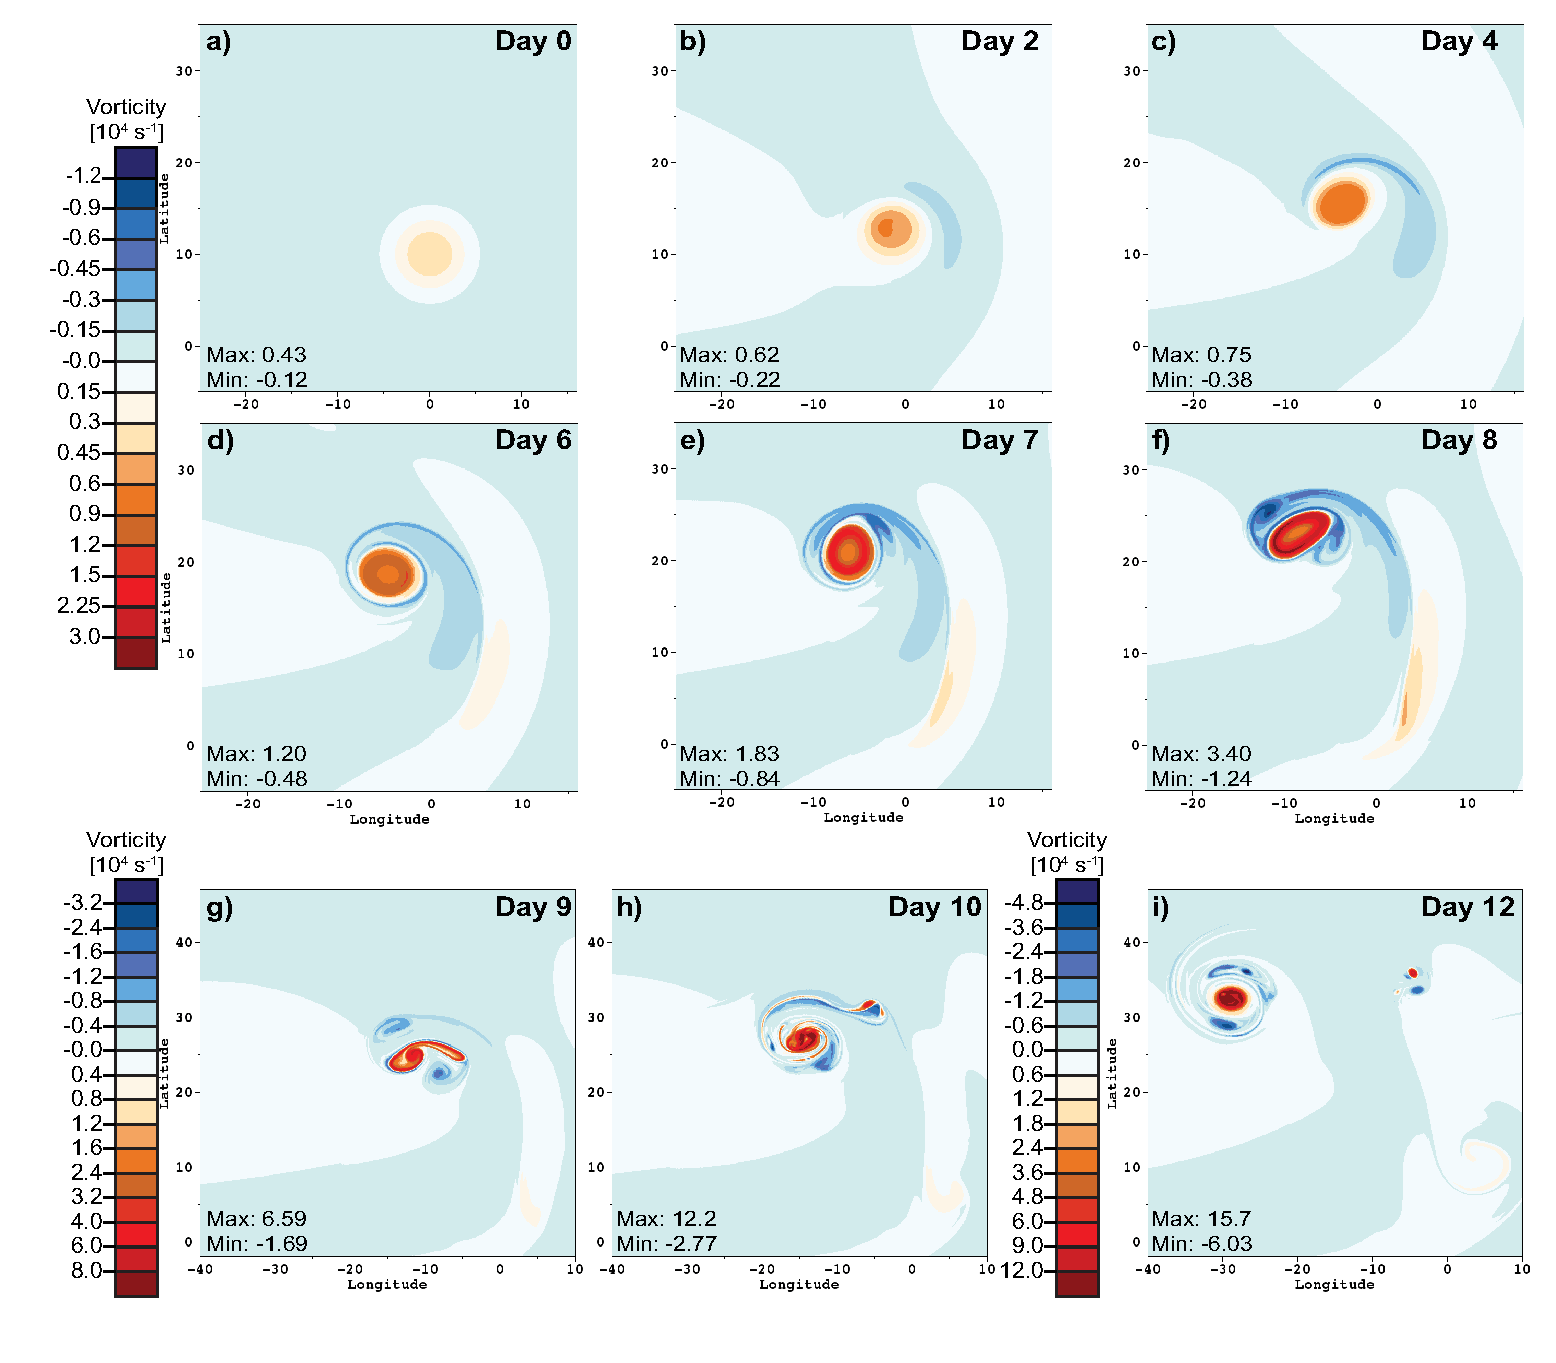
\includegraphics[width=\textwidth]{Figures/c2048_vort_intime-01.eps}}
   \caption{The evolution of the relative vorticity for an isolated strengthening vortex in a c2048 uniform run.
   (a)-(f) Relative vorticity plots for the initial condition, day 0, and days 2, 4, 6, 7, and 8 with color contour
   range of $-1.2 \times 10^{-4}$ s$^{-1}$ to $3.0 \times 10^{-4}$ s$^{-1}$. (g) and (h) Relative 
   vorticity for days 9 and 10 with the color contour ranged increased to between 
   $-3.2 \times 10^{-4}$ s$^{-1}$ to $8.0 \times 10^{-4}$ s$^{-1}$. (i) Relative vorticity for
   day 12 with a contour range of $-4.8 \times 10^{-4}$ s$^{-1}$ to $12.0 \times 10^{-4}$ s$^{-1}$.
   Note that (g)-(i) have an expanded latitude-longitude domain.}%
    \label{fig:c2048_vortseries}
\end{figure}

\begin{figure}
    \centerline{%
    \noindent
    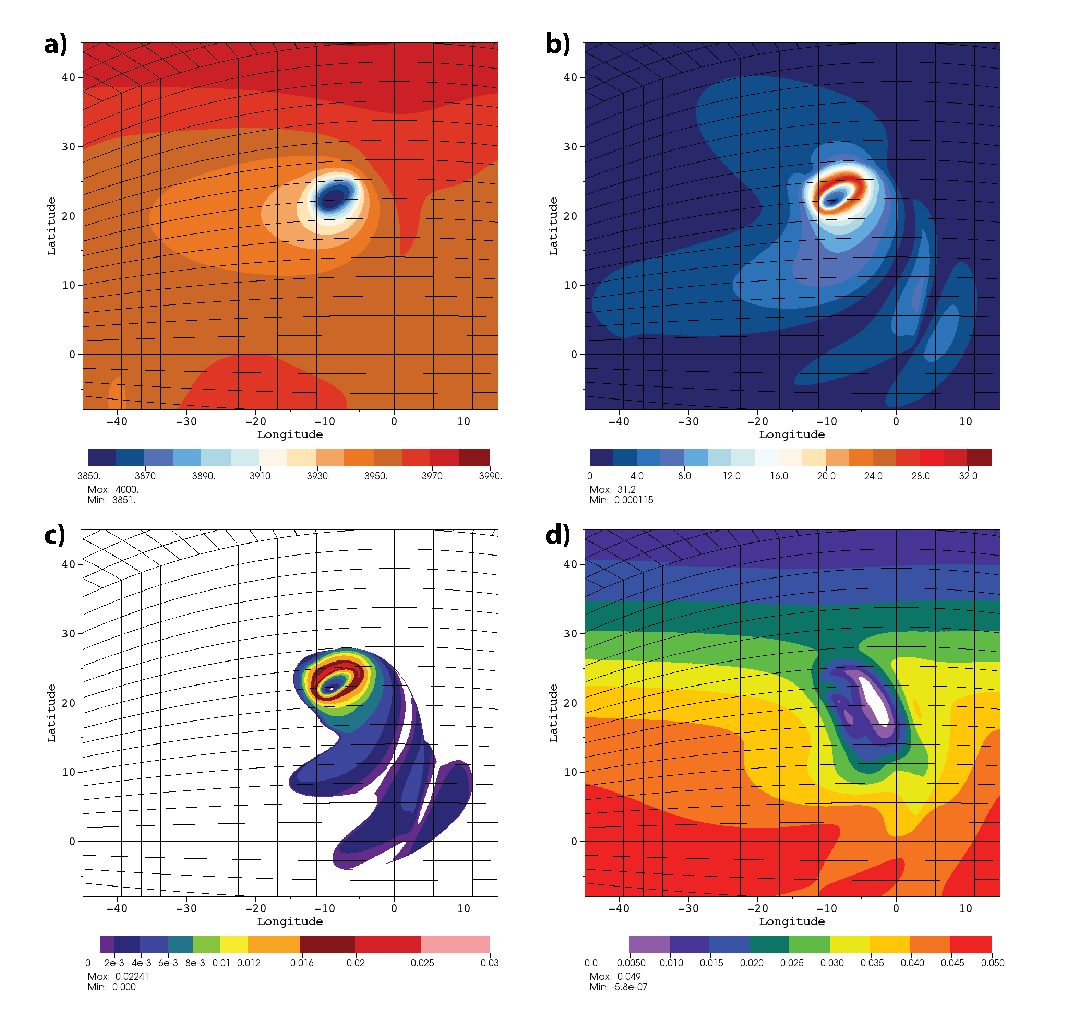
\includegraphics[width=\textwidth]{Figures/c2048_day8_plots-01.eps}}
   \caption{Day 8 plots for the uniform c2048 run of the isolated strengthening vortex for several variables: 
   (a) Height field (m), (b) Wind magnitude (m s$^{-1}$), (c) Instantaneous precipitation rate (moisture value per day), 
   and (d) Reservoir moisture content (moisture value).
   These plot correspond to the day 8 vorticity plot in Fig. \ref{fig:c2048_vortseries}(f), though
    note the larger latitude-longitude domain in these plots. }%
    \label{fig:c2048_day8}
\end{figure}

%\begin{figure}
%    \centerline{%
%    \noindent
%    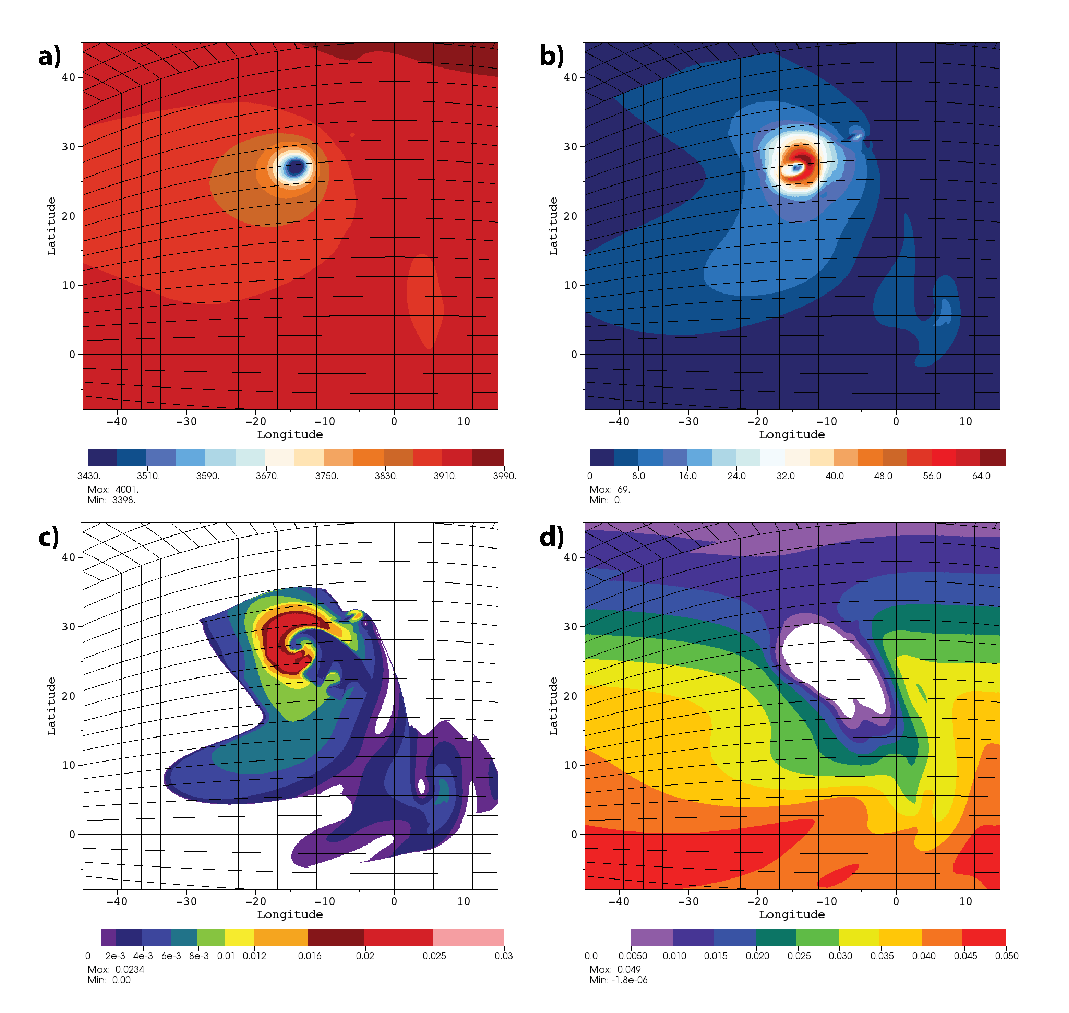
\includegraphics[width=\textwidth]{Figures/c2048_day10_plots-01.eps}}
%   \caption{Day 10 plots for the uniform c2048 run of the isolated strengthening vortex for several variables: 
%   (a) Height field (m), (b) Wind magnitude (m s$^{-1}$), (c) Instantaneous precipitation rate (moisture value per day), 
%   and (d) Reservoir moisture content (moisture value).
%   These plot correspond to the day 10 vorticity plot in Fig. \ref{fig:c2048_vortseries}(h), though
%    note the different latitude-longitude domain in these plots. }%
%    \label{fig:c2048_day10}
%\end{figure}

\begin{figure}
   \centerline{%
   \noindent
   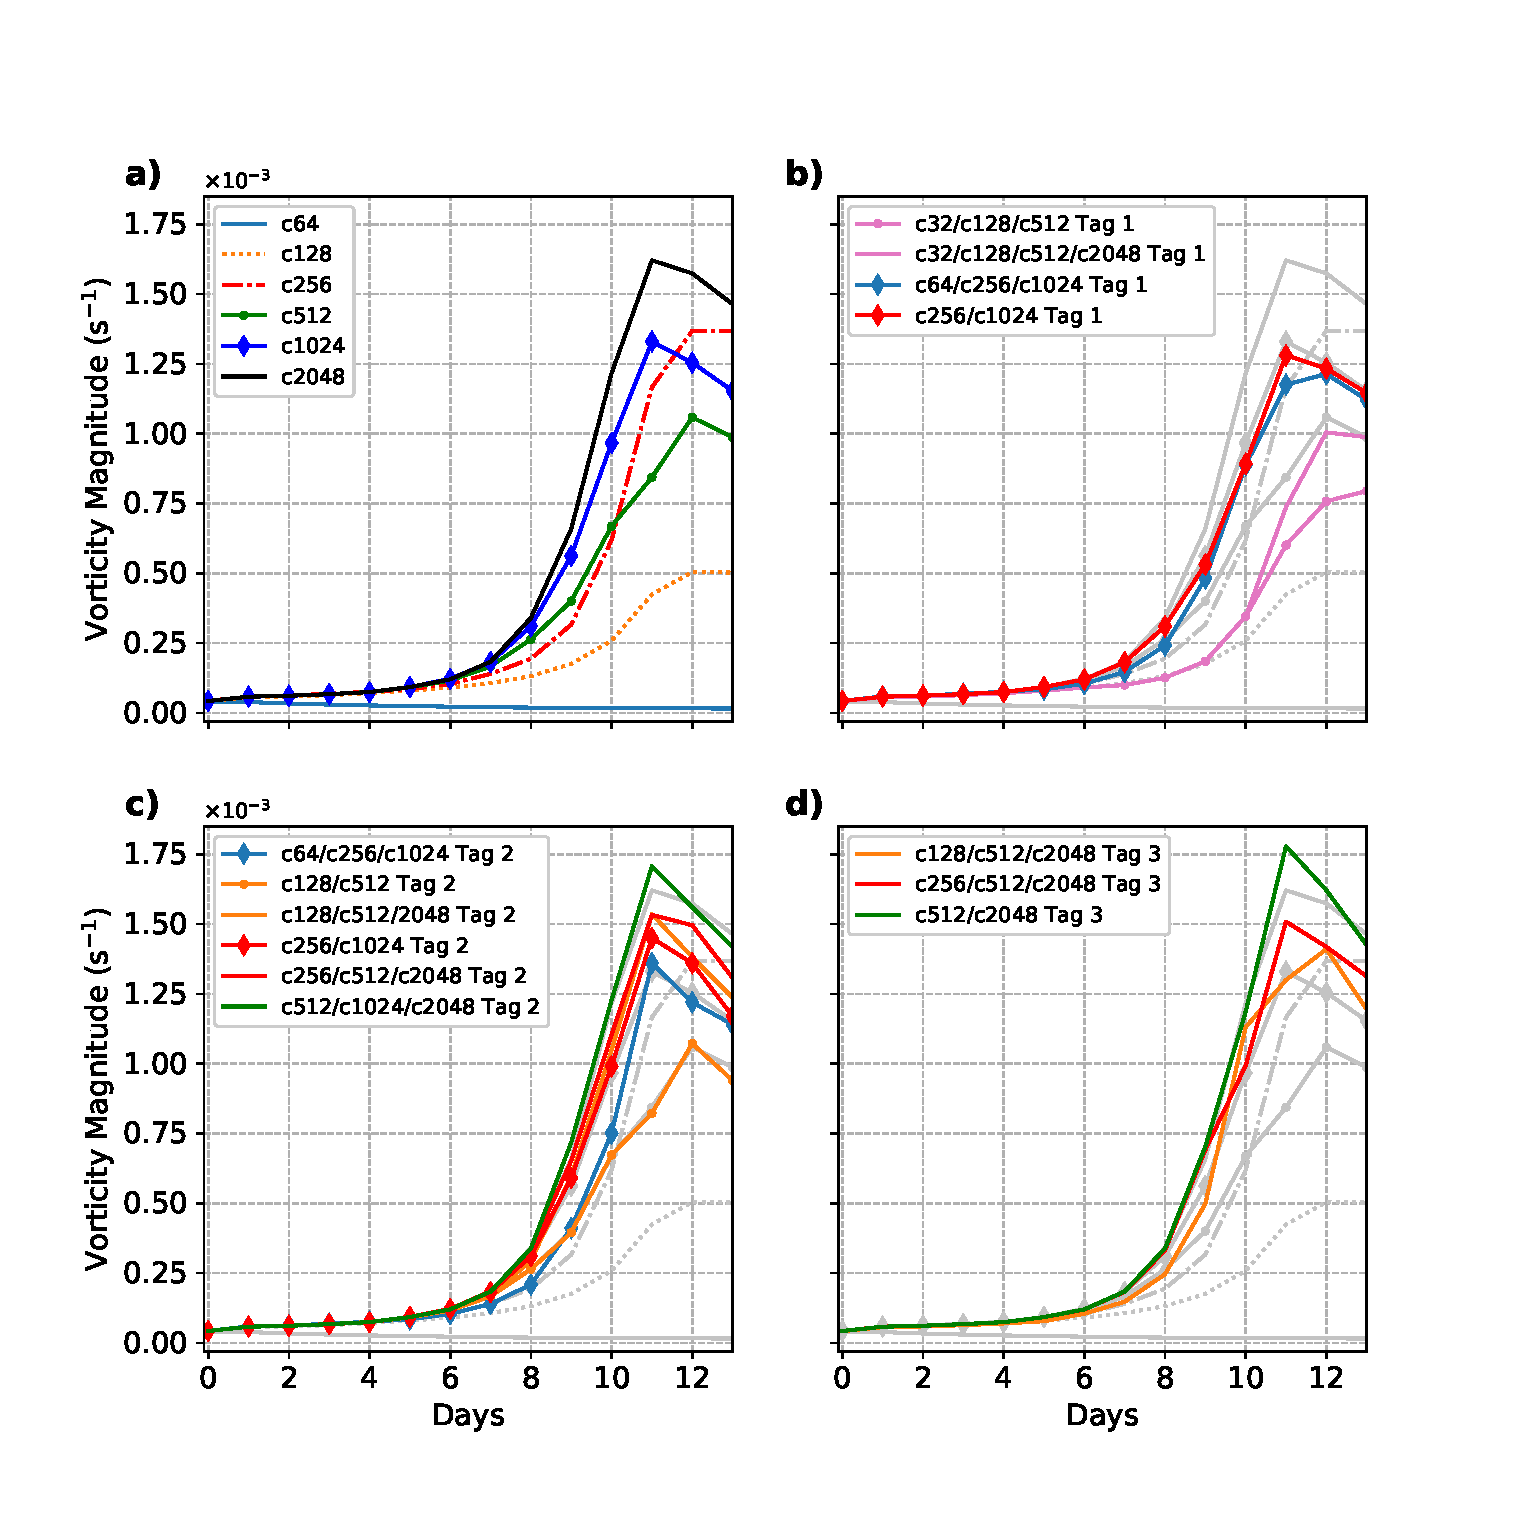
\includegraphics[width=\textwidth]{Figures/vortmax_lineplot.eps}}
   \caption{Maximum relative vorticity of the strengthening vortex over a 
   period of 13 days for (a) uniform runs, (b) AMR runs using the Tag 1
    refinement criteria, (c) AMR runs using the Tag 2 criteria, and (d)
   AMR runs using the Tag 3 criteria. For comparison purposes the 
   uniform run lines from (a) have been imposed in light grey on
   the other three plots.
   }
   \label{fig:vort_lineplot}
\end{figure}

\begin{figure}
   \centerline{%
   \noindent
   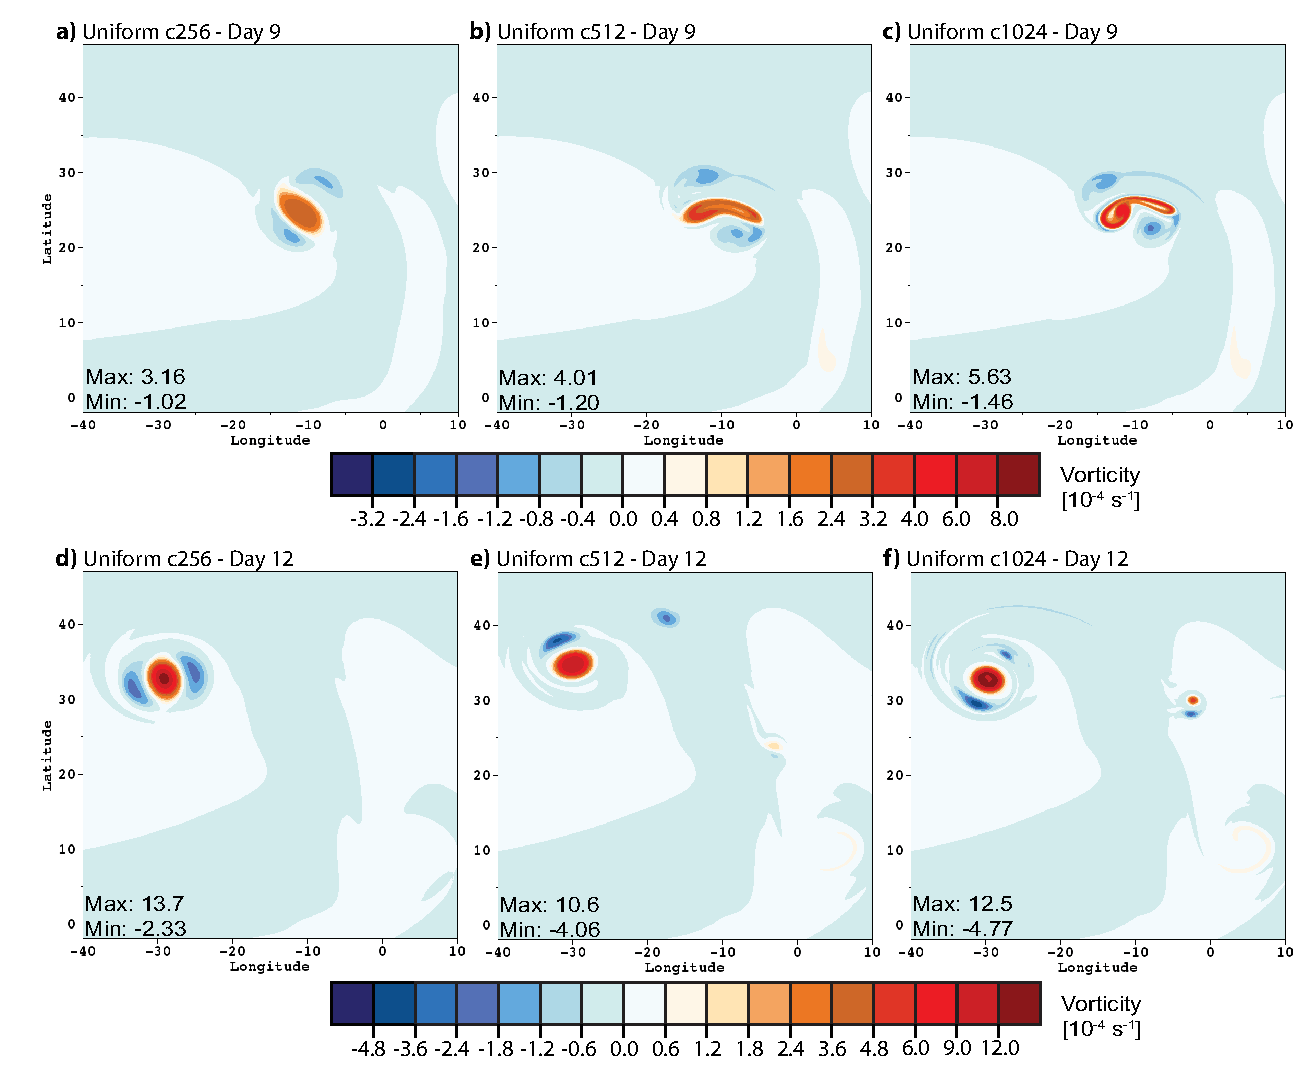
\includegraphics[width=\textwidth]{Figures/uni_runs_day9n12-01}}
   \caption{Relative vorticity field of the 
   strengthening vortex case at day 9 (a) - (c) and day 12 (d)-(f) for uniform runs 
   c256 resolution (a) and (d), c512 resolution (b) and (e), and 
   c1024 resolution (c) and (f). These plots
   correspond to the day 9 uniform c2048 plot, Fig. \ref{fig:c2048_vortseries}g, and
   day 12 plot Fig. \ref{fig:c2048_vortseries}i.
   }
   \label{fig:uni_d9nd12}
\end{figure}

\begin{figure}
   \centerline{%
   \noindent
   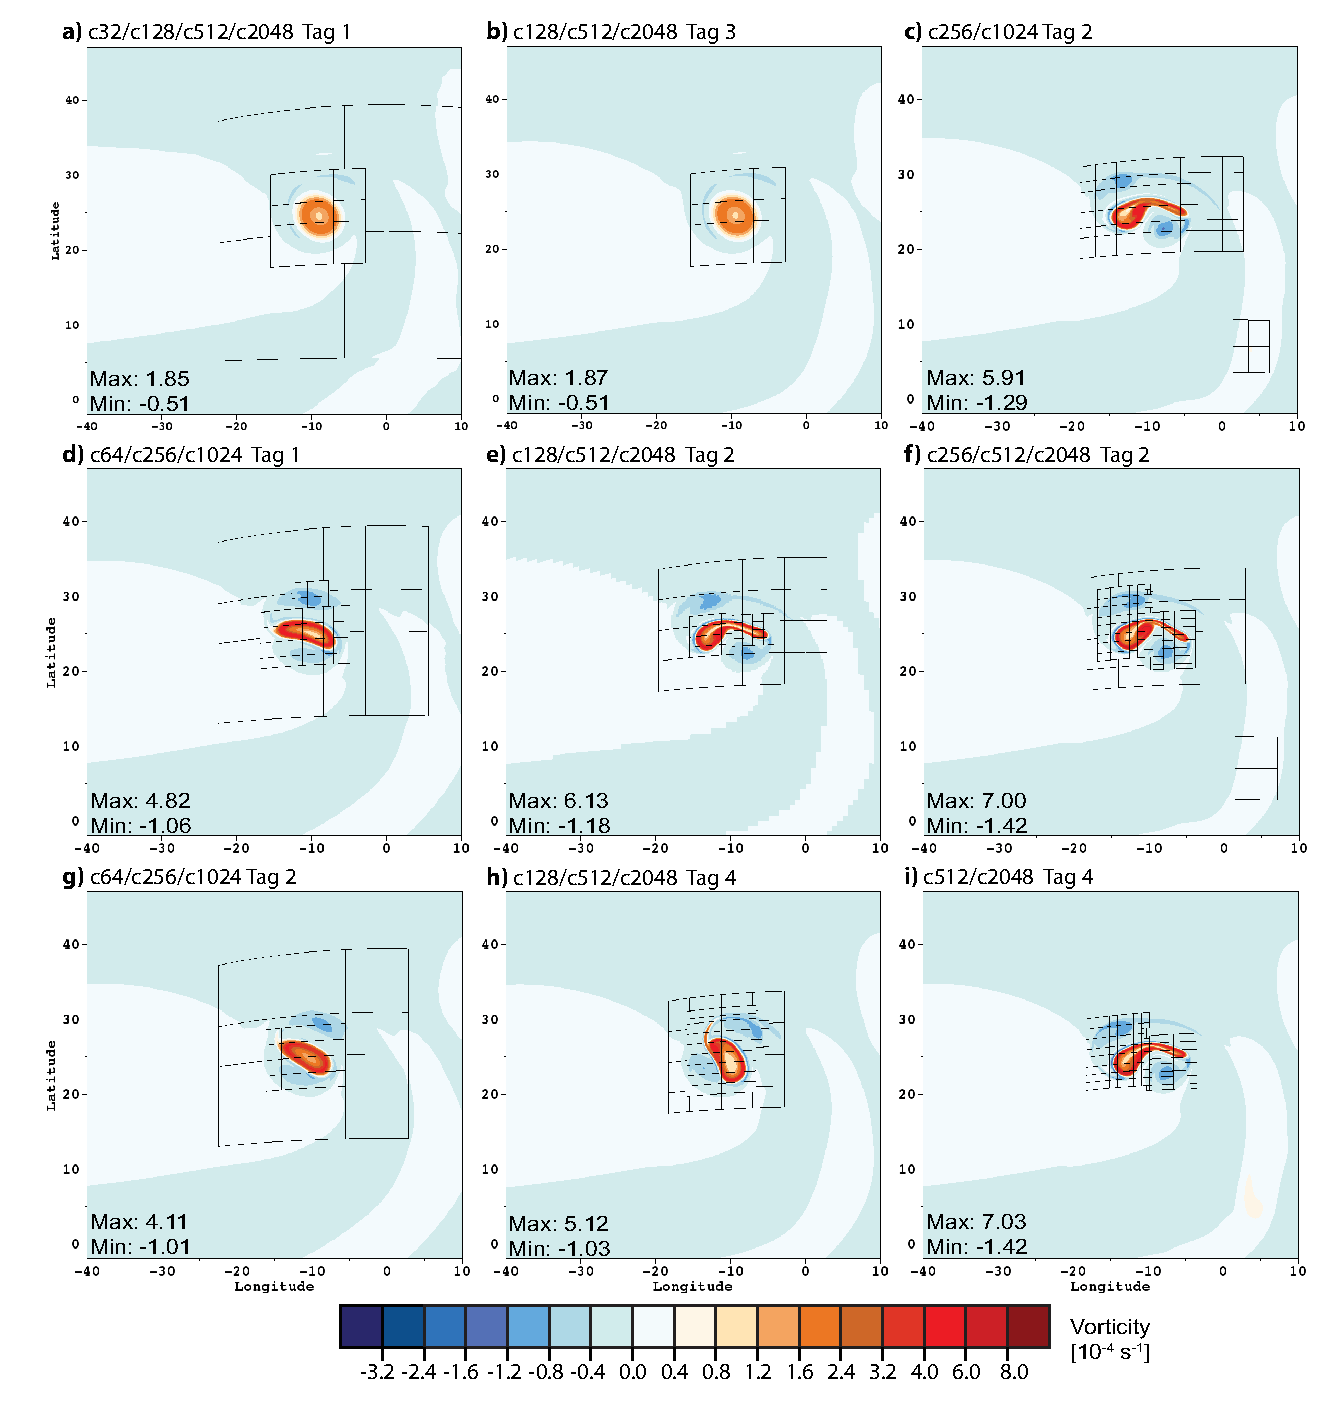
\includegraphics[width=\textwidth]{Figures/day9_vort-01.eps}}
   \caption{Relative vorticity fields at day 9 for six AMR runs of the 
   strengthening vortex case. %(a) c32 base 4-level AMR run with x4 
   %refinement using Tag 1. (b) c128 base 2-level AMR run with
   %x4 refinement using Tag 3.
   %(c) c256 base 1-level AMR run with x4 refinement using Tag 2.
   %(d) c64 base 2-level AMR run with x4 refinement using Tag 1.
   %(e) c128 base 2-level AMR run with x4 refinement using Tag 2.
   %(f) c256 base 2-level AMR run with one level of x2 refinement 
   %and one of x4 refinement using Tag 2.
   %(g) c64 base 2-level AMR run with x4 refinement using Tag 2.
   %(h) c128 base 2-level AMR run with x4 refinement using Tag 4.
   %(i) a c512 base 1-level AMR run with x4 refinement using Tag 4. 
   These plots correspond to the day 9 uniform plots in Fig. \ref{fig:c2048_vortseries}g and
   \ref{fig:uni_d9nd12}(a)-(c). The block structures of the multiple refinement
   levels are outlined in black
   }
   \label{fig:vort_amr_day9}
\end{figure}

\begin{figure}
   \centerline{%
   \noindent
   \includegraphics[width=\textwidth]{Figures/day12_vort-01.eps}}
   \caption{Same as Fig. \ref{fig:vort_amr_day9}, but for day 12 after the small
   secondary vortex has spun off. These plots correspond to the day 12 uniform
   plots in Fig. \ref{fig:c2048_vortseries}i and \ref{fig:uni_d9nd12}(d)-(f). 
   The block structures of the multiple refinement
   levels are outlined in black
   }
   \label{fig:vort_amr_day12}
\end{figure}

%\begin{figure}
%   \centerline{%
%   \noindent
%   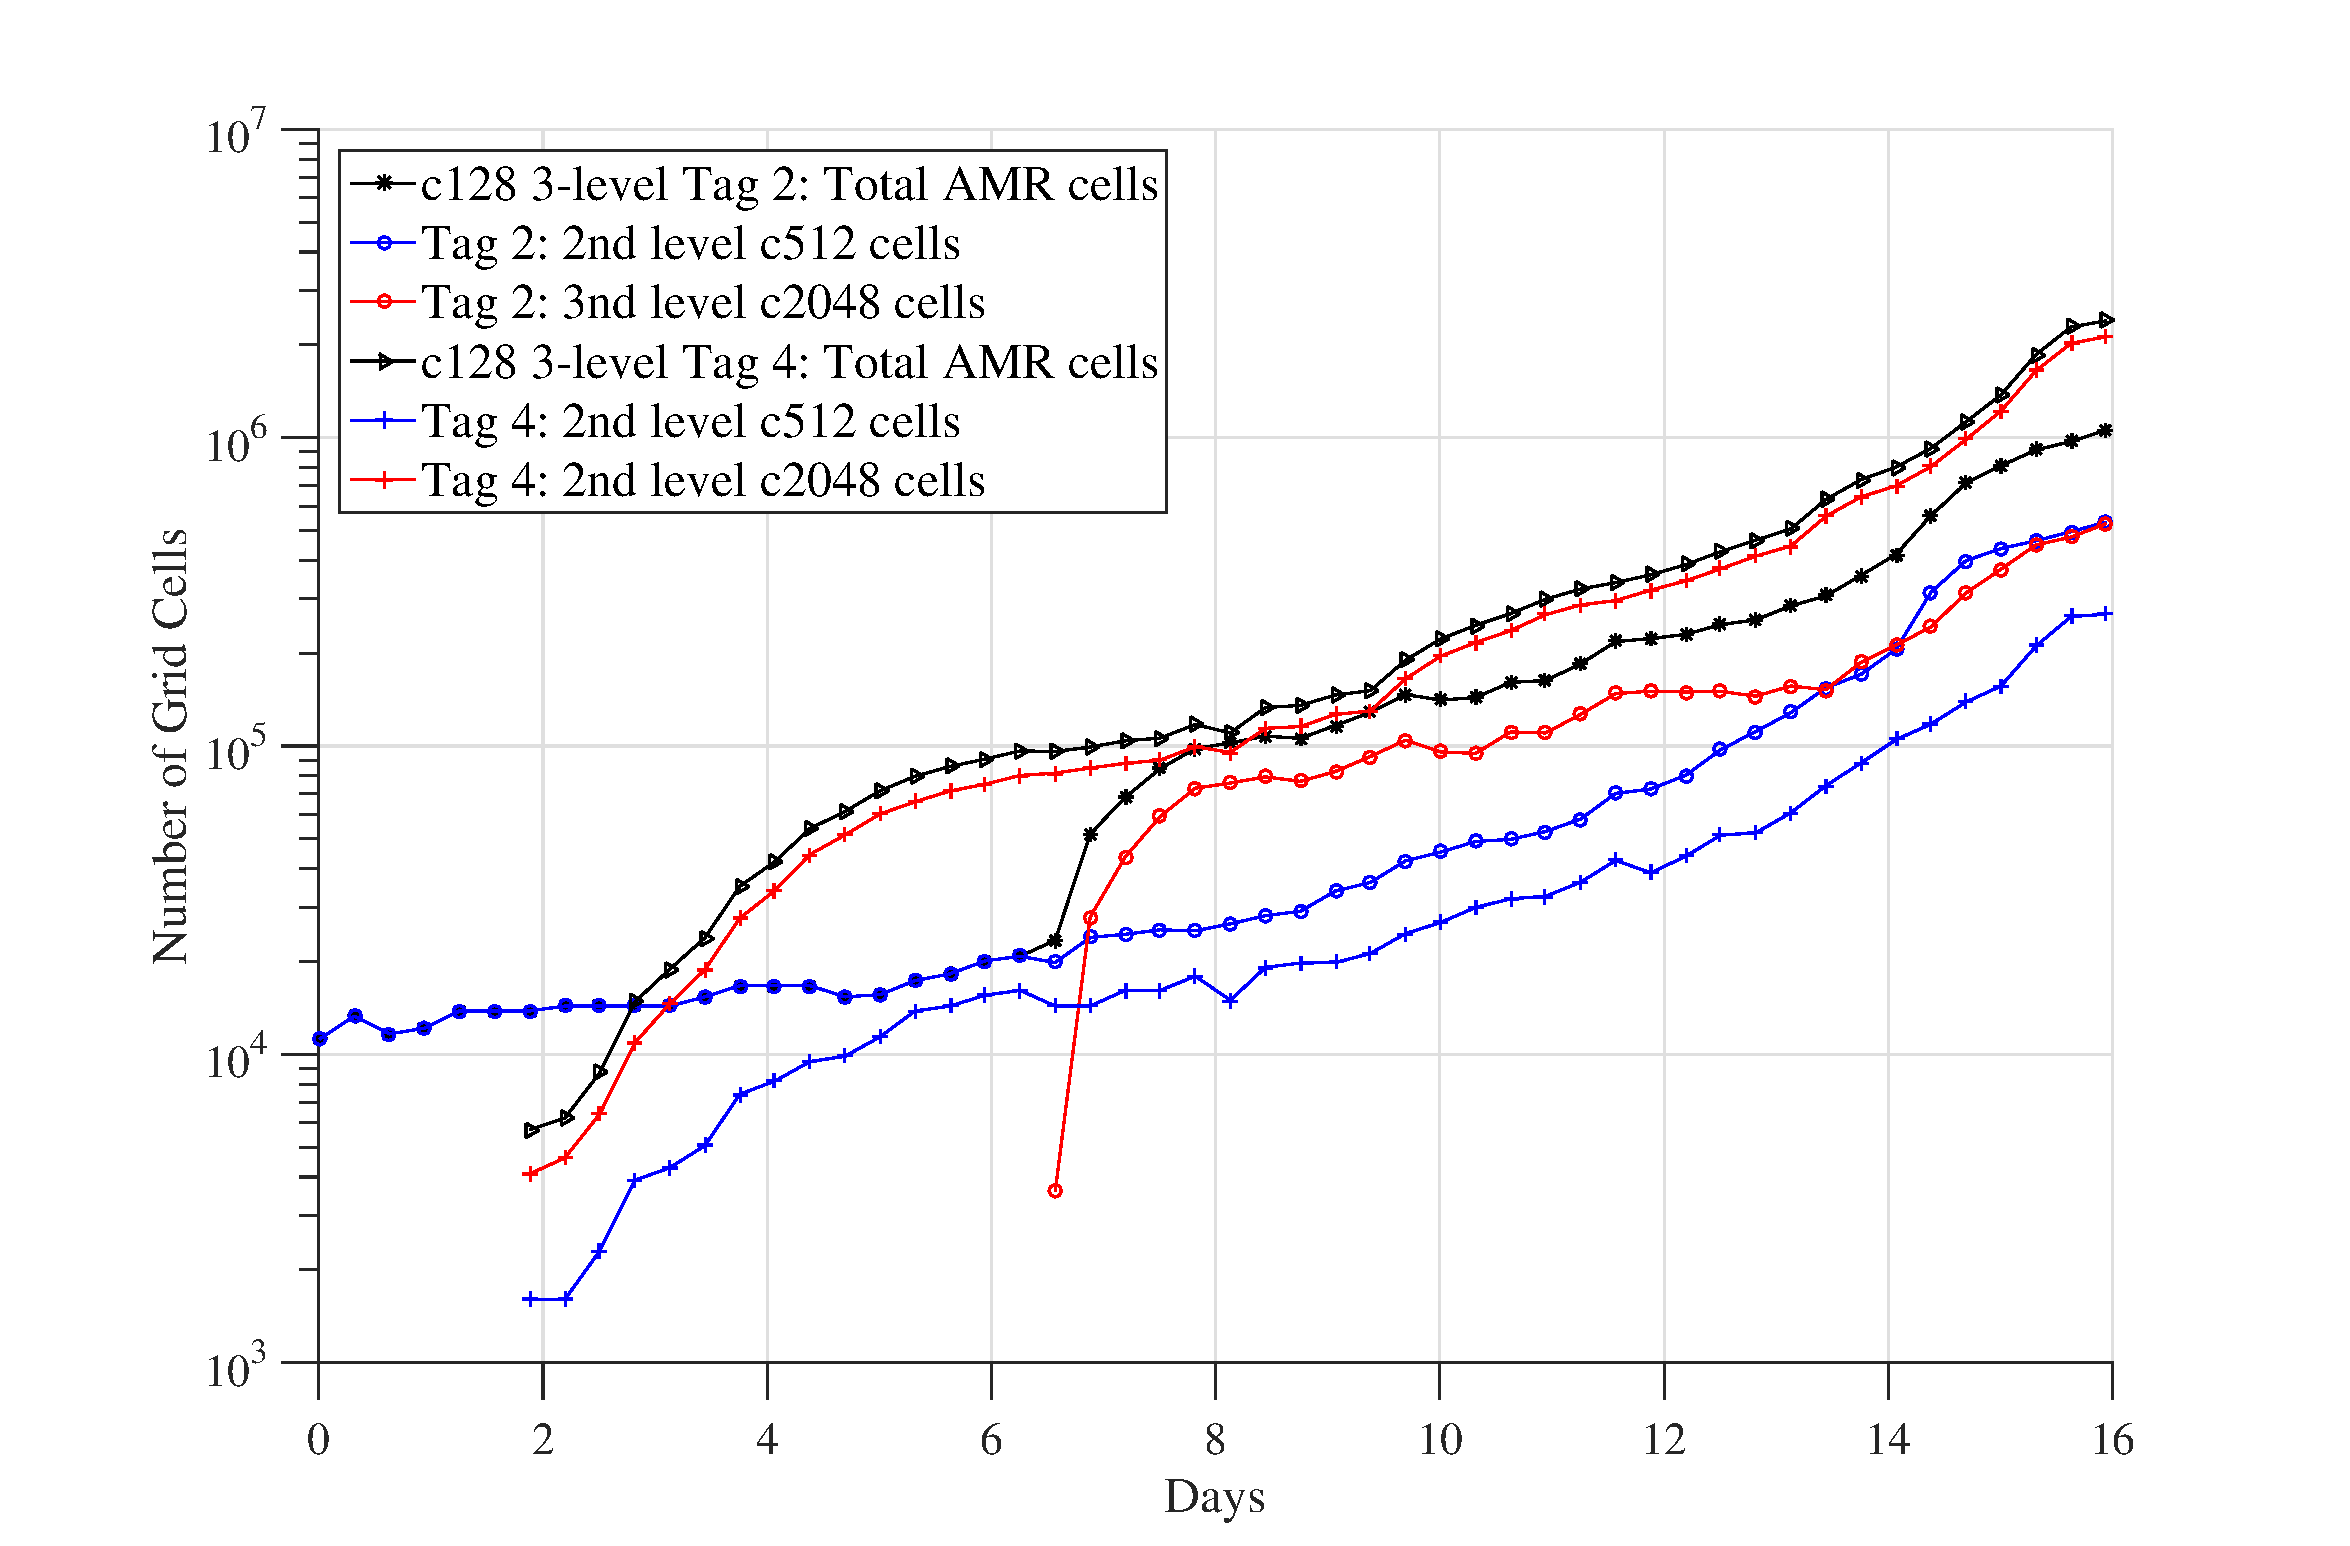
\includegraphics[width=\textwidth]{Figures/c128_3l4_Tag2vs4_compare.eps}}
%   \caption{The growth of AMR grid cells over time for the two c128 2-level AMR runs 
%   with tag 2 and tag 4 refinement criteria. The base level c128 grid cells are excluded
%   while the 2nd level c512 cells are plotted in blue and the third level c2048 cells are
%   plotted in red with a plus marker to denote the tag 4 run and a circle to denote the
%   tag 2 run.  The sum of the two levels are plotted in black with a triangle marker denoting
%   the tag 4 run and an asterisk marking the tag 2 run. 
%   }
%   \label{fig.grid_num_c128}
%\end{figure}

%\begin{figure}
%   \centerline{%
%   \noindent
%   \includegraphics[width=\textwidth]{Figures/global_uni_vort-01.eps}}
%   \caption{Late run evolution of the relative vorticity field for the 
%   strengthening vortex case with three initialized vortices. These plots show
%   the growth of a global chaotic regime by day 16 in for uniform resolution
%   runs. Relative vorticity snapshots at days 9 (left column), 12 (middle column), 
%   and 16 (right column) are given for
%   (a) uniform c256 run, (b) uniform c512 run, (c) uniform c1024 run, and
%   (d) uniform c2048 run. The leftmost vortex in the days 9 and 12 plots
%   located around $(30^\circ \mathrm{N}, 15^\circ \mathrm{W})$ is the isolated
%   vortex discussed in previous sections. The two vortices centered around
%   $(20^\circ \mathrm{N}, 90^\circ \mathrm{E})$ are the binary pair. Note: the
%   vorticity extrema occur in the isolated vortex in all cases for days 9 and 12 so they are 
%   not displayed.}
%   \label{fig:threevort_uni}
%\end{figure}

%\begin{figure}
%   \centerline{%
%   \noindent
%   \includegraphics[width=\textwidth]{Figures/day16_vort-01.eps}}
%   \caption{Relative vorticity fields at day 16 for four AMR runs of the strengthening
%   vortex case with three initialized vortices: 
%   (a) c64 base 2-level AMR run with x4 refinement using Tag 2,
%   (b) c128 base 2-level AMR run with x4 refinement using Tag 2,
%   (c) c256 base 1-level AMR run with x4 refinement using Tag 2,
%   and (d) c256 base 2-level AMR run with one level of x2 refinement 
%   and one of x4 refinement using Tag 2. The left column depicts the vorticity 
%   field at day 16 while the right column overlays
%   the block structures of the refinement levels in black. These plots
%   are comparable to the day 16 plots in Fig. \ref{fig:threevort_uni}.
%   }
%   \label{fig:vort_amr_day16}
%\end{figure}

\begin{figure}
   \centerline{%
   \noindent
   \includegraphics[height=.9\textheight]{Figures/A_c2048_allvar_zoom-01}}
   \caption{Day 6 snapshots of the evolving barotropic wave for the c2048 uniform 
   run's (a) temperature field, (b) $q_v$ moisture field, (c) $q_c$ cloud field, (d) past 12-hour 
   accumulation of the $q_r$ precipitated water field. The solid and dashed black contour
   lines in (c) and (d) represent the positive and negative relative vorticity respectively.
   The spacing between contour lines is $5 \times 10^{-5}$ s$^{-1}$.
   }
   \label{fig:c2048allvar}
\end{figure}

\begin{figure}
   \centerline{%
   \noindent
   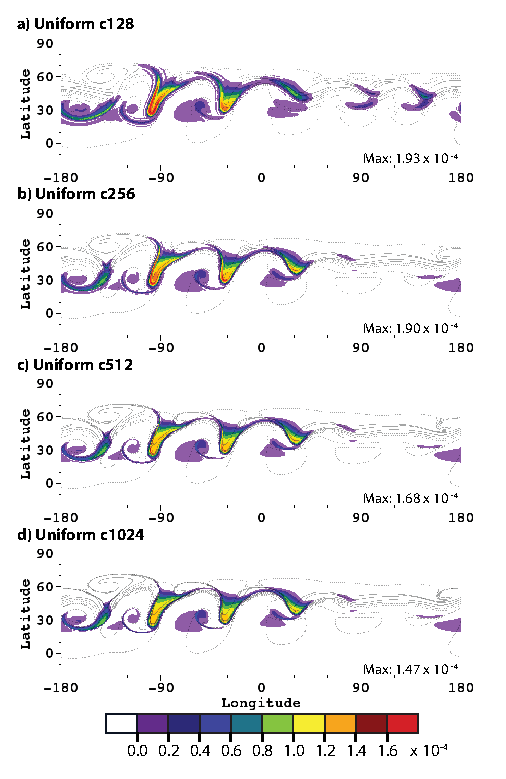
\includegraphics[height=.9\textheight]{Figures/A_qc_uniform-01}}
   \caption{Plots of the $q_c$ cloud field at day 6 for several 
   uniform resolutions: (a) c128, (b) c256, (c) c512, and (d) c1024.The c2048 uniform run
   plot of the same field in Fig. \ref{fig:c2048allvar}c serves as a reference. 
   The solid and dashed black contour
   lines represent the positive and negative relative vorticity respectively using the
   same contour spacing as in Fig. \ref{fig:c2048allvar}.
   }
   \label{fig:uniformqc}
\end{figure}

\begin{figure}
   \centerline{%
   \noindent
   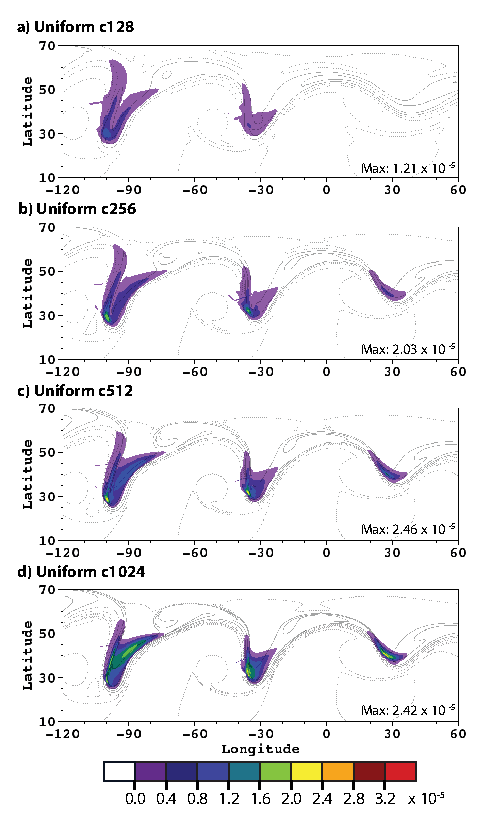
\includegraphics[width=19pc]{Figures/A_qrdt_uniform_zoom-01}}
   \caption{Plots depicting the 12-hour accumulation in the $q_r$ precipitated water field for
   (a) c128, (b) c256, (c) c512, and (d) c1024 uniform runs. The c2048 uniform run
   plot of the same field in Fig. \ref{fig:c2048allvar}d serves as a reference.
   The solid and dashed black contour
   lines represent the positive and negative relative vorticity respectively using the
   same contour spacing as in Fig. \ref{fig:c2048allvar}.
      }
   \label{fig:uniformqrdt}
\end{figure}

\begin{figure}
   \centerline{%
   \noindent
   \includegraphics[height=.85\textheight]{Figures/A_amr_qc-01}}
   \caption{The cloud $q_c$ field profile at day 6 for several AMR runs with one level of x4 refinement. 
  The tagging criterion for (a) and (d) is a relative vorticity threshold of
  $|\zeta| > 2.3 \times 10^{-5}$ s$^{-1}$. The criterion for (b) and (c) is $q_c > 3.0\times 10^{-5}$.
   The block structures of the refinement levels are outlined in black.
   }
   \label{fig:amrqc}
\end{figure}

 \begin{figure}
   \centerline{%
   \noindent
   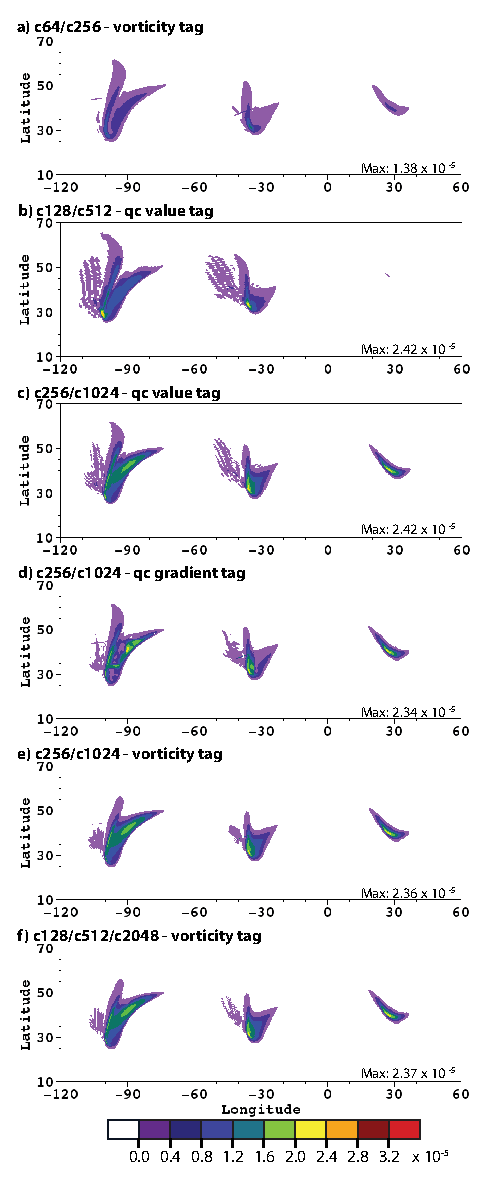
\includegraphics[width=19pc]{Figures/A_amr_qrdt_zoom-01}}
   \caption{Past 12-hour accumulation of $q_r$ at day 6 for the AMR runs depicted in Fig. \ref{fig:amrqc}.
   }
   \label{fig:amrqrdt}
\end{figure}

\end{document}